\label{sec:ttsm}

\newacronym{ttsm}{TTSM}{Time-travelling State Machine}
\newacronym{fsm}{FSM}{Finite-State Machine}
\newacronym{bim}{BIM}{Building Information Modelling}
\newacronym{ipfs}{IPFS}{Interplanetary File System}
\newacronym{cqrs}{CQRS}{Command-Query Responsibility Segregation}
\newacronym{uml}{UML}{Unified Modeling Language}
\newacronym{dto}{DTO}{Data Transfer Object}
\newacronym{oos}{OoS}{out of scope}

\definecolor{workflow_layer}{RGB}{127, 97, 26}
\definecolor{rules_layer}{RGB}{106, 127, 96}
\definecolor{persistence_layer}{RGB}{75, 97, 127}
\definecolor{consistency_layer}{RGB}{116, 91, 127}

This chapter briefly introduces the methodology used to derive an applicable concept for a \gls{bct}-based \gls{ttsm} that allows verification of \glspl{bp}. Furthermore, it discusses why this methodology has been chosen and what kind of tailoring has been applied. Afterwards, the proposed concept, as well as its software architecture, are described in detail and design decisions are discussed. The remainder of this chapter focuses on the implementation of a prototype that is later on used for evaluation of the concept.

\section{Design Science Methodology}
\label{sec:ttsm:methodology}
The concept proposed in this work was designed and developed using the design science methodology for information systems research described by Hevner et al.\ Design science, sometimes referred to as design research, is a constructive research methodology rooted in engineering and the study and evaluation of the artificial. It fundamentally is a problem-solving paradigm that aims to change the existing by creating artifacts such as constructs, models, methods, and instantiations and by providing utility. Produced artifacts are evaluated against metrics and use cases derived from a predefined (organizational) problem space in a so-called \textit{design cycle}~\cite{hevner2004_design_science}. According to Denning et al.~\cite{denning1997_design_science} and Hevner et al.~\cite{hevner2004_design_science}, design science seeks to

\begin{quote}
    ``create innovations that define the ideas, practices, technical capabilities, and products through which the analysis, design, implementation, management, and use of information systems can be effectively and efficiently accomplished.''~\cite[p.~76]{hevner2004_design_science}
\end{quote}

The problem space of efficient privacy-preserving \gls{bct}-based state machines that allow traceability, as well as the search process paved by related literature and existing business process engines, makes design science a well-fit methodology to create a novel approach for a \gls{ttsm}. The following outlines the need for a \gls{bct}-based \gls{ttsm} approach from an industrial and a research-based point of view. Furthermore, for better reproducibility of the results, the upcoming sections give an overview of the tailoring performed to the design science methodology and its guidelines, as described by Hevner et al.~\cite{hevner2004_design_science}, in order to exactly fit the needs of this work.

\subsubsection{Guideline 1: Design as an Artifact}
\label{sec:ttsm:methodology:gl1}
This work produces two distinct artifacts during the course of its design science research approach. The first one is the concept proposed for a privacy-preserving \gls{bct}-based \gls{ttsm} that allows verification of (inter-organizational) workflows and business processes in the form of an abstract software architecture and design. The second artifact is the instantiation of the aforementioned model in the form of a prototype system also used for evaluation.

\subsubsection{Guideline 2: Problem Relevance}
\label{sec:ttsm:methodology:gl2}
As stated above, recent years have not only shown an ever-growing interest in \glspl{bct} alone but also in their usage for managing workflows and \glspl{bp} due to some favorable characteristics such as fault tolerance and traceability. Nonetheless, limitations of \glspl{bct}, like block size limits, transaction limits, cost, privacy concerns, and a lack of experts, hinder businesses from adapting and using such technologies in the long run. However, they still recognize the potential of \glspl{bct} to replace trusted third parties in inter-organizational \glspl{bp} in order to not only reduce capital expenses but also create a mutual trust basis for everyone to equally participate in regardless of size or resources available~\cite{blockchains_for_bpmn_challenges_and_opportunities,blockchain_and_iot_for_bpm,impact_of_trust_on_supply_chains,untrusted_bp_execution_using_blockchain,public_chains_make_private_chains_obsolete,baseline_spec}.

\subsubsection{Guideline 3: Design Evaluation}
\label{sec:ttsm:methodology:gl3}
In chapter~\ref{sec:evaluation}, the prototype, and thus the proposed concept, are evaluated against simplified real-world \glspl{bp} (e.g.,\ the facility maintenance use case) to demonstrate its practical utility. Furthermore, qualitative and quantitative software engineering testing methodologies were employed to allow better reproducibility of results in future work, including analytical, experimental, and descriptive evaluation methods.

\subsubsection{Guideline 4: Research Contributions}
\label{sec:ttsm:methodology:gl4}
The research contributions of this work are the design artifacts. This includes the proposed concept for a \gls{ttsm} introduced in section~\ref{sec:ttsm:proposal} and the prototypical implementation as instantiation in section~\ref{sec:ttsm:prototype}. Additionally, future work can rely on the introduced \glspl{bp} for evaluation.

\subsubsection{Guideline 5: Research Rigor}
\label{sec:ttsm:methodology:gl5}
This work is based upon a formal background in \glspl{bct}, distributed systems and state machine replication~\cite{consensus_comparison_2019,nakamoto2009,ethereum_yellow_paper,impossibility_result_1985}. The formal semantics of statecharts allow for sophisticated analysis and evaluation of the proposed concept~\cite{inter_organizational_bps_managed_by_blockchain}. \gls{bpmn} and choreography diagrams are employed as a common basis for \gls{bp} specification. Furthermore, chapter~\ref{sec:related-work} provides an overview of state-of-the-art knowledge regarding formalism and pragmatism around workflow execution and state machines on the blockchain.

\subsubsection{Guideline 6: Design as a Search Process}
\label{sec:ttsm:methodology:gl6}
The \gls{bct}-based \gls{ttsm} for verifiable \glspl{bp} concept is designed by (1) performing a related work literature review of state machines and workflow execution engines on the blockchain in chapter~\ref{sec:related-work}. This step is followed by (2) deriving simplifications of real-world \glspl{bp} using requirements engineering methodologies such as requirements elicitation~\cite{christel1992_requirements_elicitation} in the form of problem scoping, understanding, and visualization using \gls{bpmn} and choreography diagrams. Thereafter, the (3) iterative search for an applicable concept is performed by evaluating different prototypical implementations for their utility against aforementioned \glspl{bp}, deriving software architecture diagrams to perform architectural analysis as well as using other analytical and experimental methods mentioned later on in chapter~\ref{sec:evaluation}.

\subsubsection{Guideline 7: Communication of Research}
\label{sec:ttsm:methodology:gl7}
The artifacts produced are described in detail in sections~\ref{sec:ttsm:proposal} and~\ref{sec:ttsm:prototype}. Additionally, chapter~\ref{sec:evaluation} provides context in the form of a simplified real-world scenario that the proposed concept is being evaluated against. This enables technology-oriented audiences to implement and extend upon the proposed concept. Furthermore, the problem statement has been described in detail in chapter~\ref{sec:introduction} to allow management-oriented audiences to determine if organizational resources should be committed.



\section{Proposed Concept}
\label{sec:ttsm:proposal}
Based on the aforementioned gap in the state-of-the-art in section~\ref{sec:related-work:comparison} and the described motivational scenario of a building administrator contracting a facility maintenance service provider in section~\ref{sec:background:bpm:bpmn}, a novel approach for a \gls{bct}-based \gls{ttsm}\footnote{Later on only referred to as \gls{ttsm}.} that allows time-travel verification of \glspl{bp} is proposed by this work. The concept aims to provide a (partially) privacy-preserving state machine that allows the definition and instantiation of workflows and the transition between states of workflows while ensuring consistency and traceability by leveraging \gls{bct}. Furthermore, it aims to provide a straightforward interaction mechanism for past workflow states. In other words, participants should be able to easily verify the correctness of a workflow's past states and state transitions.

The main objective of this chapter is to describe a \gls{ttsm} that enables off-chain workflow execution that smoothly integrates with existing blockchain solutions to make use of some of the properties of \glspl{bct}. Additionally, the concept should be integratable into existing systems of record. Before describing the concept in more detail, the goals and non-goals are clarified. This chapter does not aim to describe a concept:

\begin{table}[h]
\centering
\begin{tabular}{|c|l|c|}
    \hline
    \textbf{Code} & \textbf{Description} & \textbf{Reason} \\
    \hline
    NG1 & for a blockchain, layer-2 rollup or smart contract & \gls{bct} \\
    NG2 & that itself ensures safety and liveness properties & \gls{bct} \\
    NG3 & that itself ensures (Byzantine) fault tolerance  & \gls{bct} \\
    NG4 & that itself establishes consensus between participants  & \gls{bct} \\
    NG5 & for validating supplementary rules & \acrshort{oos} \\
    NG6 & that determines how data is persisted on the blockchain & \acrshort{oos} \\
    NG7 & that translates descriptive diagrams to \gls{ttsm} configurations & \acrshort{oos} \\
    NG8 & that determines and ensures the identities of participants & \acrshort{oos} \\
    \hline
\end{tabular}
\caption{List of non-goals for the proposed concept}
\label{tab:ttsm:proposal:non_goals}
\end{table}

Some of the declared non-goals mentioned above originate from properties blockchains ensure, and the \gls{ttsm} concept only leverages upon (indicated by reason \gls{bct}). Other non-goals are simply \gls{oos} of this work due to their significant complexity.

Instead of utilizing smart contracts or \glspl{edcc} that are directly executed on the blockchain, the proposed concept aims to create an abstraction layer for these kinds of technologies to make the system blockchain agnostic. This allows the usage of the most suitable blockchain for a given workflow. Furthermore, it permits developers to integrate yet-to-be-developed blockchains or layer-2 rollups without being vendor-locked. Not only does this increase the flexibility of possible implementations tremendously, but it also helps mitigate future security issues. In case of a newly discovered security threat in the currently used blockchain, developers can decide at any time whether the blockchain used is still suitable or if they might change to newer versions or entirely other solutions.

This, however, requires the \gls{ttsm} to keep track of its workflows while still having to provide traceability, immutability, consistency, and persistence properties at the same time. One part of the solution to this challenge is to retain all events that ever occurred in a persistent storage. Thus, an event-driven software architecture is proposed where its event bus is used for communication between modules. Each event dispatched into the event bus is permanently stored. Modules interested in these events subscribe to the event bus and execute their domain-specific logic (e.g.,\ performing validation or creating statistics). The results are either directly fed back into the event bus as events for usage in other modules or kept separated from the rest of the workflow (e.g.,\ in the form of logs inside a logging system\footnote{Using \href{https://prometheus.io/}{Prometheus} or the \href{https://elastic.co/}{Elastic Stack}, for example (links accessed on 2022-08-14)}).

Figure~\ref{fig:ttsm:proposal:macro_architecture} shows a software architecture diagram that visualizes the aforementioned macro software architecture of a \gls{ttsm}. To allow for a better separation of concerns, the architecture is split into four modules where each module is fully encapsulated by itself and only loosely coupled with others.

\begin{itemize}
    \item The \textcolor{workflow_layer}{\textit{Workflow}} module is solely concerned with the semantics of workflow execution, conversion from arbitrary process models to statecharts and optimization of such.
    \item The \textcolor{rules_layer}{\textit{Rules}} module enables supplementary (pragmatic) rules that might even span over the entire lifetime of a single workflow instantiation.
    \item The \textcolor{persistence_layer}{\textit{Persistence}} module permanently stores all workflow commands and events\footnote{Commands are actions that the users actively dispatch (e.g.,\ ``create workflow''), while events are actions that passively occurred during the execution of a software artifact (e.g.,\ ``workflow checked''). Commands are typically in present-tense, while events are in past-tense~\cite{whats_in_an_event_name}.}, that ever occurred during workflow execution.
    \item The \textcolor{consistency_layer}{\textit{Consistency}} module communicates with the blockchain and is the only module that also communicates with other participants in the workflow.
\end{itemize}

Each module materializes its own view of the data dispatched over the event bus and can consist of multiple sub-components if necessary. The architecture shown in figure~\ref{fig:ttsm:proposal:macro_architecture} can technically be extended by any number of modules that the specific domain requires.

\begin{figure}[h]
    \makebox[\textwidth][c]{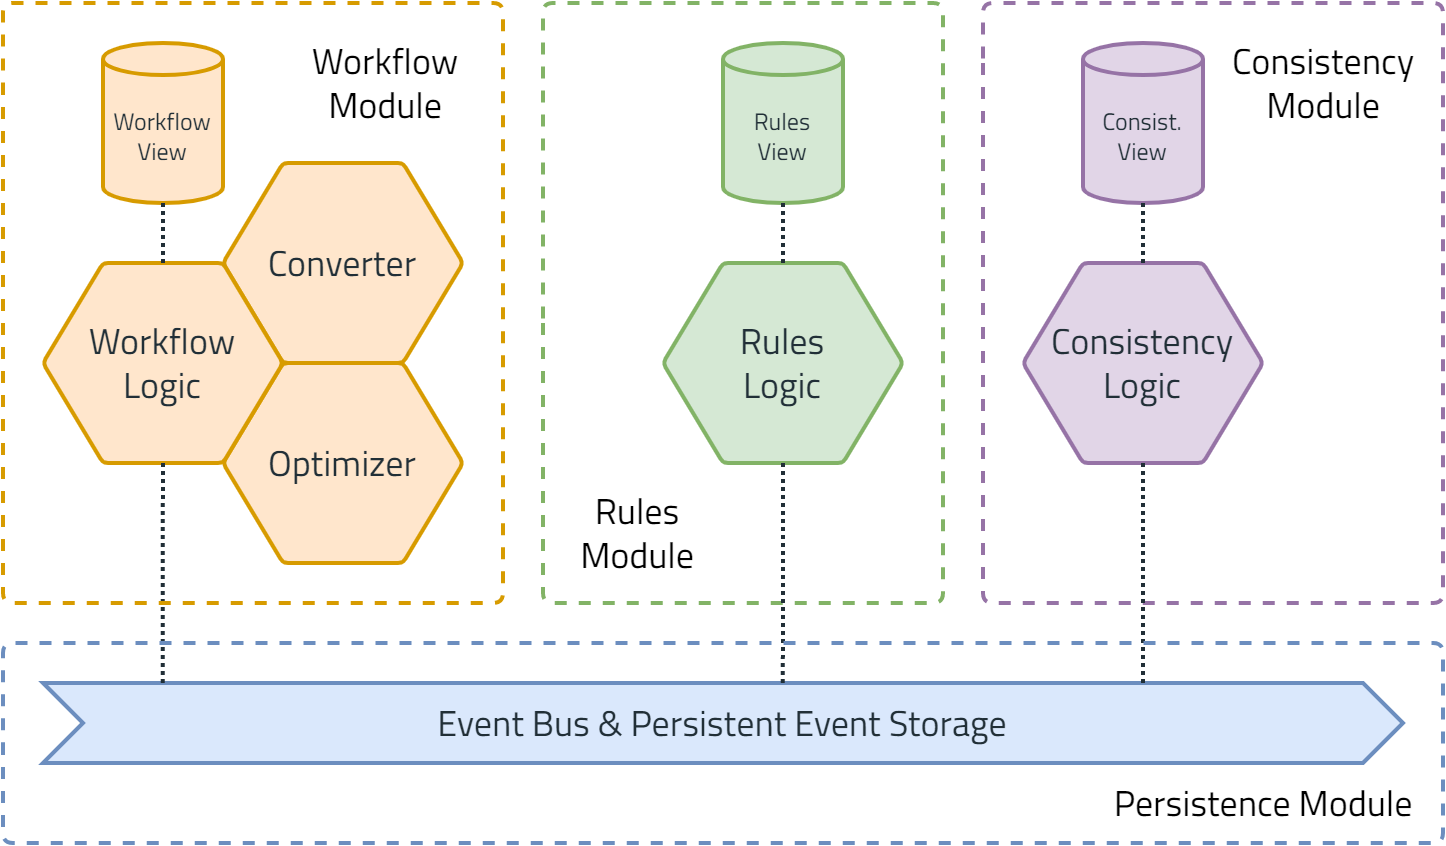
\includegraphics[width=.9\textwidth]{proposed-concept/graphics/TTSM-modules-simplified.drawio.png}}
    \caption{Macro architecture and event store design of a \gls{ttsm}.}
    \label{fig:ttsm:proposal:macro_architecture}
\end{figure}

In this software architecture, modules only communicate with each other over the event bus using predefined interfaces. It not only tries to provide a clear separation of concerns but also aims to keep stuff that changes together in close proximity to each other to improve maintainability and overall system stability. Larry Constantine, a US software engineer, shaped Constantines law, being that:

\begin{quote}
    ``A structure is stable if cohesion is high, and coupling is low.''~\cite[p.~16]{newman2019_monolith_to_microservices_constantines_law}
\end{quote}

To better illustrate the proposed concept, the remainder of this section follows along the life cycle of a single command. Commands include the creation of workflow definitions, the instantiation of workflows, and state transitions. Figure~\ref{fig:ttsm:proposal:command_life_cycle} outlines the steps that each \gls{ttsm} command has to successfully pass before consensus between participants can be reached, starting with the syntax and semantic check.

\begin{figure}[h]
    \makebox[\textwidth][c]{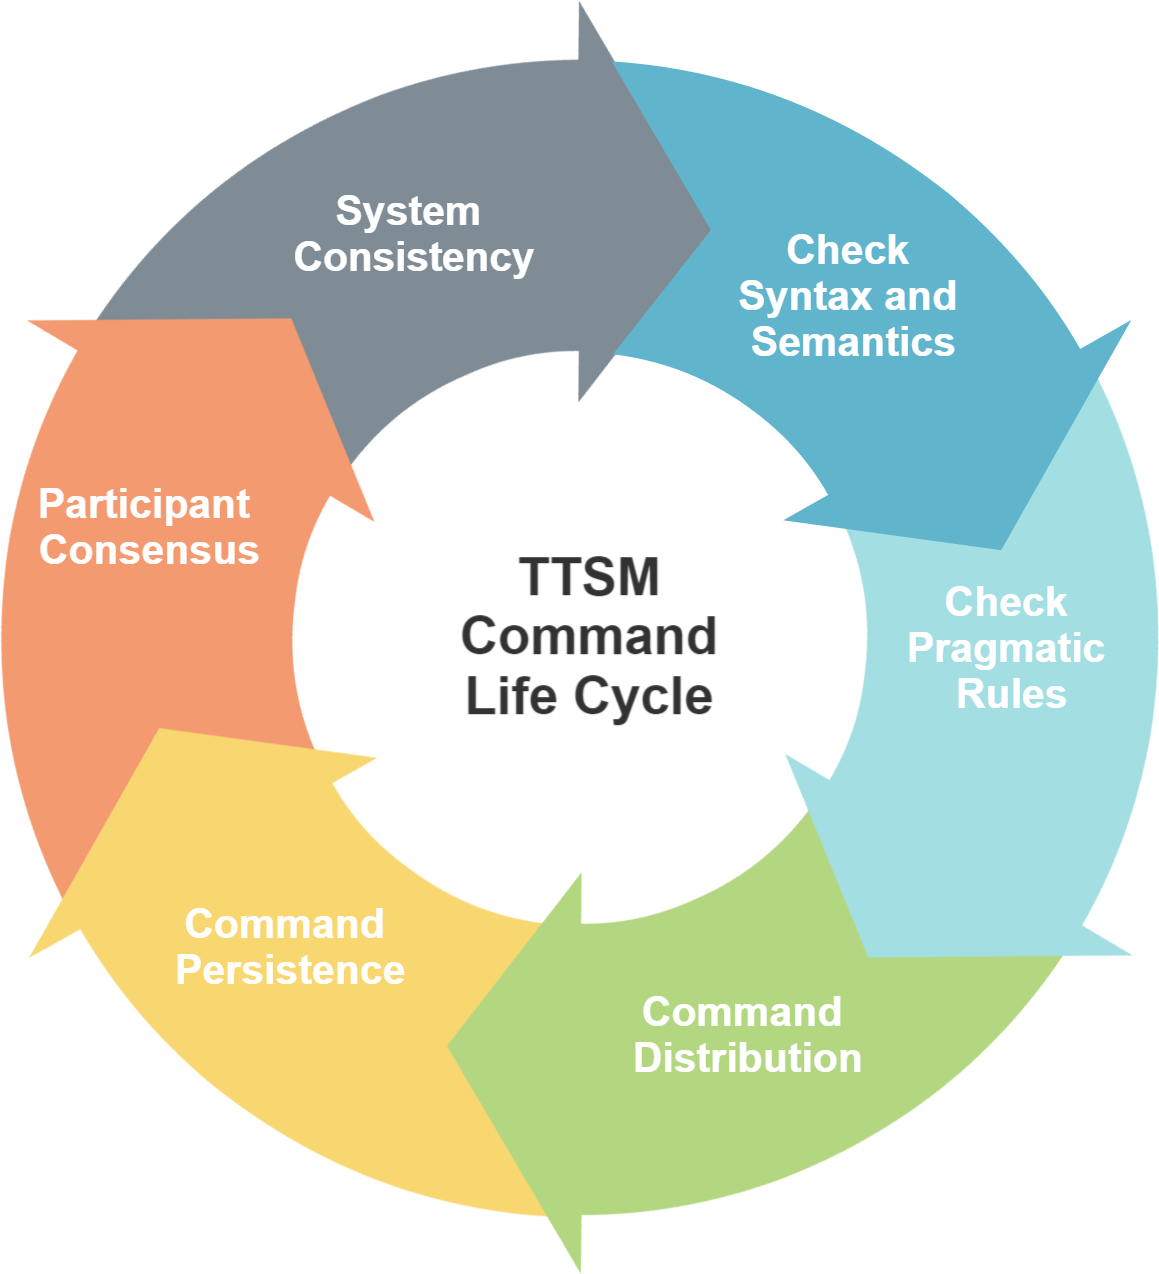
\includegraphics[width=.5\textwidth]{proposed-concept/graphics/TTSM-command-life-cycle.png}}
    \caption{Life cycle of a command dispatched in a \gls{ttsm}.}
    \label{fig:ttsm:proposal:command_life_cycle}
\end{figure}

Similar to figure~\ref{fig:ttsm:proposal:command_life_cycle}, the upcoming subsections begin with the conversion of business processes to statecharts and a check for syntactic and semantic correctness of a command. Afterwards, the rules module verifies if the command passes the employed pragmatic rules. This is followed by the distribution and persistence of the command in each participant's \gls{ttsm}. Eventually, when all participants checked and accepted the command, consensus is reached, and the system devolves into a consistent state. Note that the command life cycle is similar to the data flow in a \gls{ttsm}, where a command starts at the workflow module, passes through the rules module, and eventually reaches the consistency module. All while leaving its footprints (in the form of events) on the event bus inside the persistence module with each step. If module internal processes of defining new workflows, instantiating workflows, or performing state transitions diverge from the presented life cycle, this is stated explicitly.


%% Sender: Workflow Module
\subsection{From workflow models to statecharts}
\label{sec:ttsm:proposal:from_workflow_models_to_statecharts}
Once the participant's chosen command arrives at the workflow module, it must be converted into a statecharts-compliant format. Statecharts are used as the \glspl{ttsm} internal representation of workflows due to a vast amount of advantages, compared to \glspl{fsm}, for example, regarding workflow execution. This not only includes extensions for concurrency\footnote{An essential property for workflow execution because activities can be performed in parallel or even non-deterministic.}, but also communication between multiple participants using events~\cite{harel1987_statecharts}. Furthermore, statecharts are standardized in~\cite{statecharts_spec}, which allows developers to create appropriate tooling\footnote{e.g.,\ \url{https://xstate.js.org/} (accessed on 2022-08-15)} and the formal definition makes composition, optimization, and evaluation of statecharts more precise~\cite{inter_organizational_bps_managed_by_blockchain}. Additionally, transformation algorithms from UML sequence diagrams to statecharts~\cite{sequence_diagrams_to_statecharts} and from process models to statecharts~\cite{inter_organizational_bps_managed_by_blockchain} have been proven viable. Given the concurrency properties of statecharts, even \gls{bpmn} and choreography diagrams can be converted; however, a proof of semantic completeness for these transformations is still outstanding. Given the capabilities of statecharts and the abstraction that this transformation provides, a magnitude of modeling languages can potentially be integrated into a \gls{ttsm}. For simplicity reasons, and due to the complexity of such transformations, the remainder of this work (including the prototypical implementation in section~\ref{sec:ttsm:prototype}) assumes that participants only input statecharts compliant workflows and state\footnote{Extensions for other formats (like \gls{bpmn}) are highly encouraged to be part of future work.}.

After the transformation, the resulting statecharts are fed into the optimizer. Given a list of optimization algorithms, the \gls{ttsm} must guarantee that the specified algorithms are executed in order. A simple example of how this could be achieved is given in algorithm~\ref{alg:ttsm:proposal:ordering_optimizers}.

\begin{algorithm}
\caption{Ensure optimization algorithm order}
\label{alg:ttsm:proposal:ordering_optimizers}
\KwIn{An un-optimized statechart $s$, and a list of optimization algorithms $O$}
\KwOut{Optimized statechart $s^{\prime}$}
$s^{\prime} \gets s$\;
\ForAll{$o \in O$}
{
    $s^{\prime} \gets o(s^{\prime})$\;
}
\Return{$s^{\prime}$\;}
\end{algorithm}

Optimizers that ignore the given order can cause undesirable side effects because optimization algorithms have no means of being commutative\footnote{i.e.,\ $o_1 \circ o_2 \neq o_2 \circ o_1$}. The optimizer only runs once per workflow definition and always returns valid statecharts. There is no limitation to the amount of optimization performed; however, the semantics of the output $s^{\prime}$ should always be the same as the semantics of the input $s$. An example of such an optimization algorithm was published by Nakamura et al.~\cite{inter_organizational_bps_managed_by_blockchain} (see related work section~\ref{sec:related-work:nakamura}). Eventually, the optimization step aims to reduce the number of events emitted to the blockchain to reduce overall cost. Optimization algorithms themselves, however, are out of scope of this work. Figure~\ref{fig:ttsm:proposal:create_workflow} shows the described data and process flow inside the workflow module as sequence diagram.

\begin{figure}[h]
    \makebox[\textwidth][c]{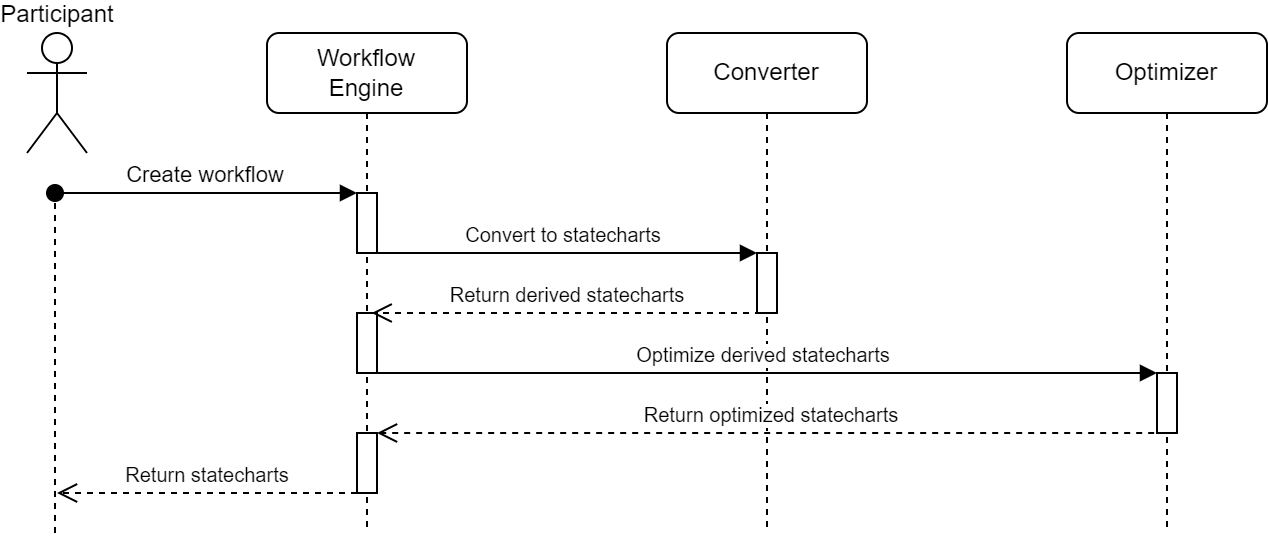
\includegraphics[width=1\textwidth]{proposed-concept/graphics/create-workflow.drawio.png}}
    \caption{Sequence diagram for the creation of a workflow definition inside the workflow module.}
    \label{fig:ttsm:proposal:create_workflow}
\end{figure}

Once optimization is complete, the workflow module checks if the given statecharts configuration is valid. Similar semantic checks are employed for workflow instantiations as well as state transitions because the state of the entire system and all workflows are known at any time and exposed by the persistence module. If the command is not allowed in the current state of the system or the workflow, it is rejected. Otherwise, it is forwarded to the event bus.


\subsection{Distinction of workflows and instantiations}
\label{sec:ttsm:proposal:distinction_workflows_instantiations}
As depicted in figure~\ref{fig:ttsm:proposal:macro_architecture}, a \gls{ttsm} is separated into four distinct modules. Clients, to be more precise \textit{workflow participants}, solely interact with the system by talking to the exposed API of the workflow module. This intended abstraction aims to hide implementation details such as the used blockchain in the consistency module or the attached rule services in the rules module. A \gls{ttsm} workflow module exposes three fundamental commands that participants can trigger at any point in time: (1) participants can propose an entirely new workflow definition with new activities and interactions between participants in the case of a choreography, (2) they can launch a new instance of a previously defined workflow definition and (3) they can initiate a state transition on a previously launched workflow instance. The separation of workflow definitions and workflow instantiations allows the association of data to a specific instantiation and thus improves flexibility~\cite{weske2012_bpm_architectures}. This is similar behavior to a lot of artifact-centric approaches such as the ones proposed by Ladleif et al.~\cite{modeling_blockchain_based_choreographies} or Lichtenstein et al.~\cite{data_driven_choreography_data_reusability_lichtenstein}. Furthermore, the separation of workflow definitions and instantiations has been shown to be rather advantageous compared to other approaches in interpreted \gls{bct}-based workflow execution engines due to the smaller footprint left behind on the blockchain itself~\cite{lean_architecture_for_blockchain_based_process_execution,interpreted_bp_on_blockchain_weber,interpreted_bp_on_blockchain_loukil}.


%% Sender: Persistence Module
\subsection{Persisting system state}
\label{sec:ttsm:proposal:capturing_local_progress}
After the successfully converted and optimized statecharts have been returned to the user for further insight, a single event is dispatched for each action to be performed (defining a new workflow, instantiating a previously defined workflow, and performing state transitions on a workflow instance) to the persistence module. The persistence module stores the entire state transition event, including its payload if present, without further processing. Technically, this allows participants to implement and add custom storage solutions without having to modifying the \gls{ttsm} itself. For large payloads, for example, state transition events may only want to reference hashes to more domain-specific databases\footnote{Such as \href{https://speckle.systems/}{Speckle} for \gls{bim} data or the \gls{ipfs}~\cite{interplanetary_file_system} as content-addressable storage (links accessed on 2022-08-21)}~\cite{weber2019_architecture_for_dapps_blockchain_patterns,eberhardt17off_block}.

Storing state transition events (and commands in general) persistently is of utmost importance for a \gls{ttsm}. All kinds of events dispatched in the system represent a delta $\Delta$ (or difference) that advances a particular workflow state and, therefore, the overall system state\footnote{Imagine a counter that adds one to the current value each time the user presses a button. In this scenario, $+1$ is the $\Delta$ to the current state, which in this case, is a counter $c$ that is initialized with $0$.}. Besides \textit{delta events}, there also exist \textit{fact events} that tell the system in which state a particular sub-state has been at a certain point in time. Unlike \textit{delta events}, \textit{fact events} are not used in \glspl{ttsm} because they can only be undone by entirely deleting them. On the other hand, when using \textit{delta events}, one can define an inverse operation\footnote{Recall the counter example from before. The inversion of the $+1 \Delta$ would be the $-1 \Delta$.}, which allows jumping forwards and backwards in time without modifying the event log itself. Therefore, the sum of commands (including state transitions or workflow instantiations) represents the current state of the system~\cite{fact_vs_delta_event_types,event_sourcing_and_cqrs}.

So-called event-driven software architectures not only allow time travel but also promote loosely coupled sub-systems and enable even better scalability. In other words, dispatched events do not require to be captured and processed by anyone. This allows modules to write events on a more fine-grained level and only consume data that is required. Additionally, due to the already employed event bus system, event sourcing can be used effectively and efficiently to create projections from the stored events and thus derive not only workflow critical information (such as the current state of a workflow instance) but also meta-data around the execution of workflows and the \gls{ttsm} itself. Furthermore, the event bus allows \glspl{ttsm} to be split into multiple microservices\footnote{One microservice per module.} if necessary. Not only can this improve scalability and availability, but also maintainability of the entire system dramatically~\cite{event_sourcing_and_cqrs}.

Due to the already employed event bus, a \gls{ttsm} aims to strictly separate between actions that modify the state and actions that solely accumulate and read the state to improve security and flexibility. Therefore, the persistence module embraces the \gls{cqrs}\footnote{\url{https://en.wikipedia.org/wiki/Command-query_separation} (accessed on 2022-08-21)} pattern as one of its design principles. At its core, \gls{cqrs} aims to separate database reads from database writes (i.e.,\ a question should not alter the state of the system)~\cite{meyer1988_effeil_and_cqs}. Separating reads from writes further improves scalability because each state transition allows an arbitrary payload with an arbitrary data structure to be attached. This means that the output of the event sourcing stage (i.e.,\ the current or any past state of a workflow instance or the system itself) can permanently be stored using a suitable database technology that is optimized for reads, for example. Event sourcing, combined with \gls{cqrs}, furthermore enables asynchronous communication with external services. To put this into the perspective of a \gls{ttsm}, participants can advance the state independently from a blockchain's required block transaction time (which can be up to 20 minutes on some blockchains~\cite{nakamoto2009}). Nonetheless, the system must expect rollbacks if workflow instances are advanced without confirmation from the rules or consistency module.


%% Sender: Time-Travelling
\subsection{Travelling through time}
\label{sec:ttsm:proposal:travelling_through_time}
The persistence module is the part of the system that enables time-travelling due to its event sourcing and \gls{cqrs} capabilities. If participants want to check if a specific event occurred or a workflow instance has fulfilled a particular property, all they have to do is (a) either search for this specific event by traversing all dispatched events forwards or backwards or (b) replay all previously dispatched events until a certain point in time is reached. The following exemplary list of events is used to better visualize this concept:

\begin{enumerate}
    \item[\textbf{E1}] \textbf{(12:00)} -- Create workflow $W$
    \item[\textbf{E2}] \textbf{(12:10)} -- Create workflow instance $I$ of workflow $W$
    \item[\textbf{E3}] \textbf{(12:20)} -- Perform state transition from state $A$ to state $B$ on $I$
    \item[\textbf{E4}] \textbf{(12:30)} -- Perform state transition from state $B$ to state $C$ on $I$
\end{enumerate}

If participants want to know, what the state of workflow instance $I$ was at 12:25, they have to replay all events that happened before or precisely at 12:25 in the correct order. Given the example above, this includes E1, E2, and E3. If participants want to know if a state transition from state $A$ to state $B$ happened prior to the state transition from state $B$ to state $C$, they have to go back in time and check if they can find appropriate events in the expected order (i.e.,\ E3 has to have happened before E4).

To allow these kinds of time-travelling capabilities, the \gls{ttsm} and the persistence module have to ensure \textit{causal ordering} for all events dispatched. This means that some event $A$ has to happen before another event $B$ can even occur - they are \textit{causally ordered}~\cite{causal_ordering}. In the example given above, event E2 can only occur after event E1 has occurred because the creation of a workflow instance requires a workflow to exist in the first place, and thus, they are \textit{causally linked}. A formal representation of this circumstance is given in equation~\ref{eq:ttsm:proposal:causal_order}.

\begin{equation}
\label{eq:ttsm:proposal:causal_order}
A \longrightarrow B
\end{equation}

Since \glspl{ttsm} ensure \textit{causal ordering}, reliable transitive relations can be derived. The persistence module knows that certain events must occur before others. An example of such a transitive relation of events is given in equation~\ref{eq:ttsm:proposal:transitive_relation}:

\begin{equation}
\label{eq:ttsm:proposal:transitive_relation}
(A \longrightarrow B \wedge B \longrightarrow C) \implies A \longrightarrow C
\end{equation}

Hence, one can express the transitive relation of events in a \gls{ttsm} as a relation $T$ over the set of events $E$ in first-order logic as follows:

\begin{equation}
\label{eq:ttsm:proposal:transitive_relation_over_ttsm_events}
\forall a, b, c \in E : (aTb \wedge bTc) \implies aTc
\end{equation}

This is an assumption that the \gls{ttsm} concept and its corresponding persistence module rely upon that allows consistent replaying of events, enhanced rule checking, and more in-depth optimizations before and during workflow execution.


%% Sender: Rules Module
\subsection{Validating workflow rules}
\label{sec:ttsm:proposal:validating_workflow_rules}
After the persistence module has eventually stored the events, the rules module consumes them. As mentioned above, this module enables participants to create supplementary and often more pragmatic rules for the entire workflow. In other words, when the workflow module checks if state transitions can be performed based on given statecharts, the rules module checks if state transitions can be performed based on previous state transitions and payloads attached. Since the rules module can directly communicate with the persistence module, it can also time-travel and check, for example, if certain state transitions have been performed or if the payload, which was previously attached to one of the state transitions, fulfills certain criteria\footnote{Specifying these criteria is up to the participants themselves, because they are very much domain specific.}.

As depicted in figure~\ref{fig:ttsm:proposal:macro_architecture}, the rules module communicates with external rule engines via a predefined interface. This interface allows the registration of rule engines that are triggered as soon as the participant proposes a new workflow definition, workflow instance, or state transition. The rules defined by the rule engines must all be unconditionally \textit{true}. If one or more rules cannot be checked due to unexpected circumstances (e.g.,\ a network timeout or the rule check returns an incomprehensible result), the rule check is evaluated to \textit{false}. A more formal representation can be found in equation~\ref{eq:ttsm:proposal:rules_module_success_criteria}. If the set of registered rule engines $R$ is empty, the \textit{rules valid} function $RV(t)$ is immediately evaluated to \textit{true}:

\begin{equation}
\label{eq:ttsm:proposal:rules_module_success_criteria}
RV(t) = \top \wedge \bigwedge_{r \in R} check(r,t)
\end{equation}

Each successful, failed, or erroneous response of $check(r,t)$ is re-emitted to the persistence module as a new event to allow for better traceability. This allows the executing participant to better trace configuration or network errors if, for example, one registered rule engine always fails for one specific state transition. After a response has been received from all registered rule engines, another event has to be emitted, which is created by the rules module, to indicate that the action to be performed is indeed allowed according to all previously defined rules. An exemplary algorithm for checking a state transition is provided in~\ref{alg:ttsm:proposal:rules_checking}.

\begin{algorithm}
\caption{Rules checking algorithm}
\label{alg:ttsm:proposal:rules_checking}
\KwIn{A state transition $t$, and an unordered set of registered rule engines $RE$}
$a \gets \top$\;
\ForAll{$re \in RE$}
{
    $v \gets check(re, t)$\;
    \eIf{$v$ is valid}
    {
        $emit(valid(re, v, t))$\;
    }
    {
        $a \gets \bot$\;
        $emit(invalid(re, v, t))$\;
    }
}
\eIf{$a = \top$}
{
    $emit(all\_valid())$\;
}
{
    $emit(some\_invalid())$\;
}
\end{algorithm}

In this algorithm, the variable $a$ is used as a tracking variable to flag if at least one rule check failed. If this is the case, the function $emit$ writes the event $some\_invalid$ to the persistence module to inform other modules of the failed rule check and allow better traceability later on. Compared to the optimizer, which is part of the workflow module, the rules module does not have to ensure ordering. This is because the overall validity check of a state transition shown in equation~\ref{eq:ttsm:proposal:rules_module_success_criteria} is commutative due to the properties of the \textit{logical and} ($\wedge$) operator.

Building upon the definition of the rules module, the number of events emitted per action can be computed using the total amount of rule engines registered $|RE|$. Each rule engine produces exactly one event, and an additional event is dispatched by the rules module after all rule checks have been performed. This circumstance is depicted in equation~\ref{eq:ttsm:proposal:number_of_rl_tx_per_action}:

\begin{equation}
\label{eq:ttsm:proposal:number_of_rl_tx_per_action}
EC_{rl}(RE) = |RE| + 1
\end{equation}


%% Sender: Consistency Module
\subsection{Sending workflow commands and ensuring consistency}
\label{sec:ttsm:proposal:entering_blockchain_and_distributing_commands}
Once the rules have been checked and the appropriate events dispatched, the consistency module consumes these follow-up events. In a \gls{ttsm} without a rules module (technically possible due to loose coupling), the consistency module might directly consume workflow events. One of the requirements that a consistency module in a \gls{ttsm} has to fulfill is multi-chain support because of the rapidly changing ecosystem of \glspl{bct}. Therefore, it has to provide some abstraction that allows the usage of different consistency strategies. In a \gls{ttsm}, this might be achieved by relying on the behavioral \textit{strategy design pattern}. This pattern allows the exchange of an algorithm during run-time without changing the interface~\cite{geirhos2015_design_patterns_behavioral}.

Combined with the approach proposed by Nakamura et al.\ in~\cite{inter_organizational_bps_managed_by_blockchain}, where a shared state machine and one for each participant are derived from a given workflow definition, and the approach proposed by Ladleif et al.\ in~\cite{architecture_for_multi_chain_bp_ladleif} for multi-chain support in workflow engines, the consistency module enables the usage of different blockchains not only in different workflow instantiations or definitions but also depending on the payload attached to state transitions, for example. Therefore, if participants agreed upon using different blockchains for different message types prior to workflow execution, the module can choose the applicable strategy implementation during runtime. As an example, the module might rely on an Ethereum-based strategy for larger \gls{bim} models, where only the hash of the model and a signature that proves that all relevant participants have seen the model is stored on the blockchain, while it might switch to a Baseledger-based strategy if documents must be proven correct using zero-knowledge. This, however, requires participants to agree on certain \glspl{bct} for certain use cases.

If an appropriate strategy has been chosen, the consistency module dispatches the message to all participants involved in the state transition. However, all messages must have at least one participant as recipient. This ensures that the internal workflow activities of one participant are not exposed to other participants. In such a case, the consistency module might even choose a noop\footnote{no operation} strategy to immediately feed back the message to the sender to prevent any network utilization at all and, thus, ensures separation of the shared state machine from the participants one.

Even though the strategy implementations can diverge, the messages exchanged always follow a strict format which is depicted in figure~\ref{fig:ttsm:proposal:consistency_message_format}.

\begin{figure}[h]
    \makebox[\textwidth][c]{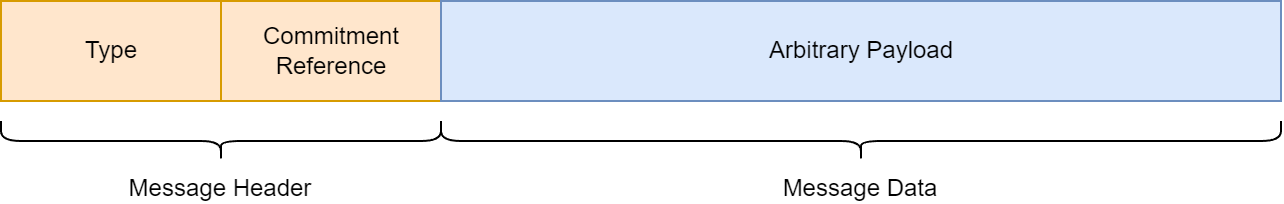
\includegraphics[width=.9\textwidth]{proposed-concept/graphics/consistency-message-format.drawio.png}}
    \caption{Format of a consistency message exchanged by participants.}
    \label{fig:ttsm:proposal:consistency_message_format}
\end{figure}

This rather simplistic configuration is split into two distinct sections: (1) the message header, which contains a unique type identifier in the form of a text string and a commitment reference that references the location where the message is stored (e.g.,\ a \gls{zkp} when using the Baseline Protocol, or a transaction reference for Ethereum or Bitcoin). (2) the message data contains an arbitrary payload using an arbitrary data structure. This might be a Base64-encoded file or even just some JSON data, for example. Depending on the message, the payload block might also contain meta information. In the case of a state transition, it stores not only the attached payload but also a unique identifier for the workflow instance on which the state transition is performed upon, the current state, the transition event name, and the expected state. Figure~\ref{fig:concept:multiple_participants} shows an exemplary setup of multiple \glspl{ttsm} to illustrate message flow between participants:

\begin{figure}[h]
    \makebox[\textwidth][c]{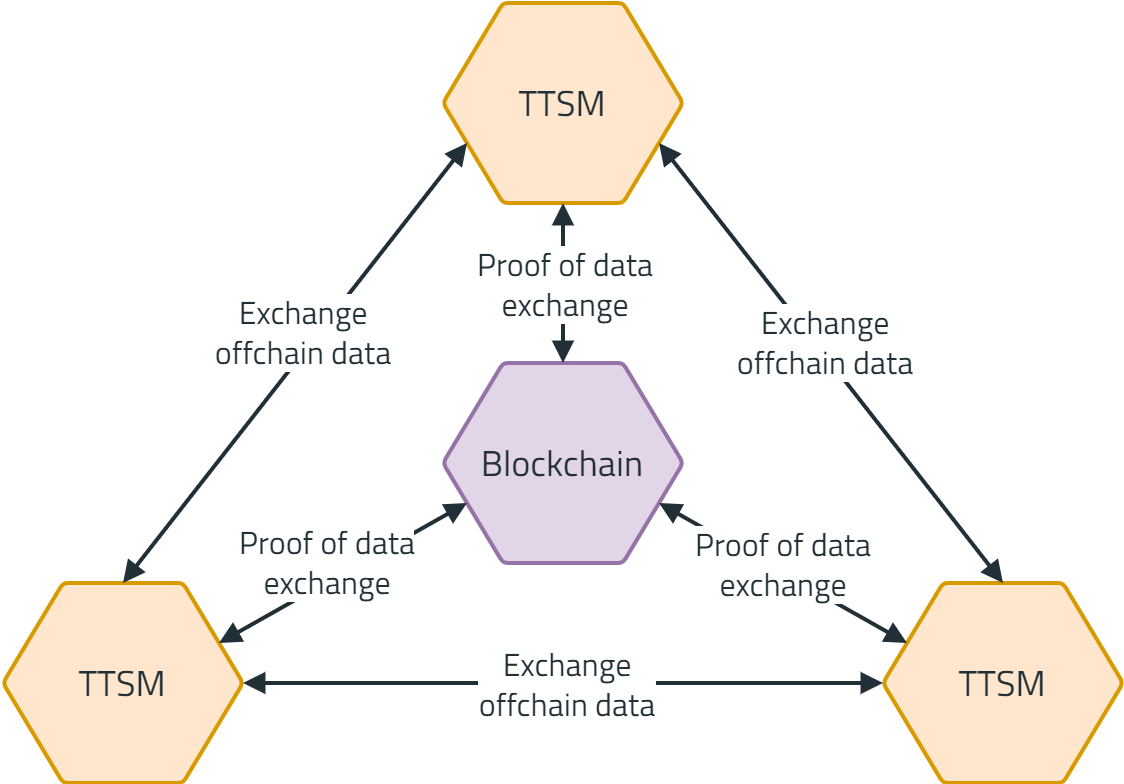
\includegraphics[width=.7\textwidth]{proposed-concept/graphics/TTSM-multiple-participants-2.drawio.png}}
    \caption{Setup of multiple \glspl{ttsm} with counterparties interacting with each other.}
    \label{fig:concept:multiple_participants}
\end{figure}

Every participant has her own instance of a \gls{ttsm}. Each \gls{ttsm} communicates with other \glspl{ttsm} by sending messages through the consistency module (by establishing TCP connections, for example). It is also the only module that directly communicates with the blockchain, in order to provide data consistency between participants.


%% Receiver: Consistency and Rules Module
\subsection{Processing workflow commands from other participants}
\label{sec:ttsm:proposal:receiving_commands}
After a connection has been established (in one way or the other, depending on the implementation of the consistency module), a message has to be dispatched to all \textit{relevant} participants of a state transition. Participants that receive this message dispatch an internal event containing the payload, the action to be performed on the workflow instance, and the commitment reference (see section~\ref{sec:ttsm:proposal:entering_blockchain_and_distributing_commands}). This ensures that all participants have undeniable proof of what happened in which order.

It is important to notice that the internal events of the \gls{ttsm} used in the persistence module are \textbf{NOT} the same events (or messages) dispatched in the consistency module and transmitted (over the blockchain) to other participants. For more complex business processes, this enables that not every single process step (including internal activities) must be written to the blockchain. This is a design constraint of the \gls{ttsm} proposal. Therefore, there can only be, at most, as many consistency events dispatched as there are persistence events. In other words, each consistency event dispatched must have at least one corresponding internal persistence event being dispatched afterwards. However, not every internal persistence event must be distributed to all other participants. This circumstance is depicted more formally in equation~\ref{eq:ttsm:proposal:comparison_bc_tx_and_events_per_transition}, where $CEC_{total}$ refers to the total number of consistency events dispatched, and $PEC_{total}$ to the total number of persistence events processed internally by the \gls{ttsm}.

\begin{equation}
\label{eq:ttsm:proposal:comparison_bc_tx_and_events_per_transition}
CEC_{total} \leq PEC_{total}
\end{equation}

After receiving the message and converting it into an internal persistence event, each \gls{ttsm} of each participant has to perform two checks:

\begin{itemize}
    \item \textbf{Syntax and semantics verification}: This check is performed by the workflow module on the transmitted data. This ensures that no incorrect state transitions, workflow definitions, or workflow instantiations can be injected by potentially hostile participants.
    \item \textbf{Rules verification}: The rules module, if present, has to perform a pragmatic verification of not only the transmitted data and its payload but also if the command is allowed in the current context regarding previously performed state transitions and their payloads. As mentioned afore, the rules module has the ability to time-travel to perform these checks.
\end{itemize}

This two-step process is the same for every command performed, even if it only regards internal workflow activities. Therefore, a participant sending a command to other participants has to perform the syntactic, semantic, and rules verification twice. Once before the consistency module transmits the command to other participants and a second time after receiving her own command. This redundant verification check ensures that commands are correctly written to the blockchain and transmitted over the network. Furthermore, it guarantees consistency because all participants work with the same commands and payloads, regardless of being sender or receiver. After verifying the command, participants generate an acceptance or rejection response. This response must be sent to all involved participants.

\begin{itemize}
    \item \textbf{Acceptance}: The participant accepts the command and advances her own \gls{ttsm} accordingly.
    \item \textbf{Rejection}: The participant rejects the command because either the syntax and semantics, the rules check, or both have failed. Denying a command restores the previous state.
\end{itemize}

If neither of both responses is sent, other participants cannot further advance their state. Handling these error cases is up to the implementation. Notice that these acceptance or rejection responses do not wait for user input. The response is entirely determined by the \gls{ttsm} internally. This means that \glspl{ttsm} do not directly support user-based decisions in workflows (e.g.,\ by asking a user in an appropriate UI if she accepts a state transition given a certain payload). However, this is entirely by design. Such user-based decisions must be modeled as part of the workflow definition itself. Statecharts, and other modeling languages that can be transformed to statecharts (such as \gls{bpmn}, for example), already include decision elements as an integral part of their specification. Therefore, user input must be handled purely declaratively on the workflow definition level by the participants themselves and is not the responsibility of the \gls{ttsm}. In other words, if a document must be shared or a decision has to be made, an applicable gateway or task must be added to the workflow.


%% Sender and Receiver: Consistency and Persistence Module
\subsection{Eventually reaching consensus}
\label{sec:ttsm:proposal:reaching_consensus}
Once a response has been sent by an involved participant\footnote{Notice that the distinction between command sender and receiver is no longer relevant at this point.}, she has to wait until all other participants have sent their responses as well. A command that concerns $N$ participants produces at most $N$ responses. At this point, the \gls{ttsm} has to handle one of three scenarios:

\begin{itemize}
    \item \textbf{Acceptance from all participants involved}: All participants accepted the command and advanced their state accordingly. Thus, consensus has been reached, and the execution of the command is complete.
    \item \textbf{Rejection from at least one participant involved}: One or more participants rejected the command and restored their previous state. Thus, all other participants must also restore their previous state to assure consistency across all parties. In other words, a rejection from at least one participant rolls back the entire command for all participants involved.
    \item \textbf{No response from at least one participant involved\footnote{See FLP impossibility result in section~\ref{sec:background:flp}.}}: This work is not concerned with this case in particular because it highly depends on implementation details and non-functional requirements such as availability, reliability, resiliency, or fault tolerance, for example.
\end{itemize}

Given these three scenarios, especially the second one is prone to attacks from hostile participants because they can deny a command infinitely many times. This threat, however, is more of a theoretical attack. Similar to the Nothing-at-Stake attack described in section~\ref{sec:background:pos}, hostile participants lose more than their potential victims. Other participants are fully aware of who rejects and who accepts commands due to the strong traceability properties of \glspl{ttsm}. Thus, the credibility of these participants suffers in the long term.

The algorithm of the consistency module, which determines the outcome of a command, is rather similar to algorithm~\ref{alg:ttsm:proposal:rules_checking} described in section~\ref{sec:ttsm:proposal:validating_workflow_rules} used to determine if a command passes the rules module. The \gls{ttsm}-consensus algorithm~\ref{alg:ttsm:proposal:consensus} is concerned with the first two scenarios described above:

\begin{algorithm}
\caption{\gls{ttsm}-consensus algorithm}
\label{alg:ttsm:proposal:consensus}
\KwIn{A command $c$, and the number of involved participants $N$}
$a \gets \top$\;
\ForAll{$i \leftarrow 1$ \KwTo $N$}
{
    $r \leftarrow next\_response()$\;
    \eIf{$r$ is acceptance}
    {
        $emit(accepted(c, r))$\;
    }
    {
        $emit(rejected(c, r))$\;
        \If{$a = \top$}
        {
            $emit(some\_rejected())$\;
        }
        $a \gets \bot$\;
    }
}
\If{$a = \top$}
{
    $emit(all\_accepted())$\;
}
\end{algorithm}

Once again, $a$ is used as a tracking variable to flag if at least one participant rejected the command. In this case, two internal events are emitted: (1) a $rejected$ event that contains not only the commitment reference but also the participant and the command itself and (2) a $some\_rejected$ event that is immediately dispatched afterwards to indicate that the command must be rolled back and the previous state restored. The algorithm, however, does not stop after one participant rejected the command. This is because all rejection responses should also be stored locally as internal events in the persistence module for better traceability.

\glspl{ttsm} leverage on the concept of ``soft state'', which means that data might be inconsistent between participants for a certain amount of time but eventually reaches consistency when things have settled~\cite{vogels2009_eventually_consistent}. This is due to the handling of participants that do not respond immediately and the block transaction time of \glspl{bct}. However, after all involved participants accepted the command, consensus has been reached and consistency archived. Therefore, the order of commands is typically determined by the consensus algorithm of the chosen \gls{bct}. Even though \glspl{ttsm} have to deal with soft state and rollbacks of commands, this single source of truth takes care of command ordering and establishing consistency between all participants.



\section{Prototype Design}
\label{sec:ttsm:prototype}
In contrast to the previous section~\ref{sec:ttsm:proposal}, this section describes a practical implementation of the proposed concept that is used for evaluation later on. Notice that not all functionalities that are theoretically possible in a \gls{ttsm} are implemented to their full extent in this prototype because it only serves as proof of concept. The prototype described uses state-of-the-art technologies and well-established industry standards to show that it is possible to implement a fully functional \gls{ttsm} leveraging on existing know-how. The upcoming sections describe a potential implementation of each module of a \gls{ttsm}. This diverges from how section~\ref{sec:ttsm:proposal} described the overall concept because this section focuses more on implementation details compared to the interoperability of the individual modules. The prototype described here is available on Zenodo\footnote{\href{https://zenodo.org/badge/latestdoi/521292268}{10.5281/zenodo.7375788} (accessed on 2022-11-29)} and GitHub\footnote{\url{https://github.com/danielkleebinder/ttsm-prototype} (accessed on 2022-11-29)}. It makes use of the following technologies:

\begin{itemize}
    \item \textbf{Node.js 16.14\footnote{\url{https://nodejs.org/} (accessed on 2022-11-29)}}: A runtime for JavaScript, built on top of the V8 JavaScript engine. It is used as an execution environment for the \gls{ttsm} itself because its event-based design makes it a good fit for systems that heavily communicate asynchronously with other systems.
    \item \textbf{npm 7.8.0\footnote{\url{https://npmjs.com/} (accessed on 2022-11-29)}}: A package manager for JavaScript and Node.js that handles dependencies using a centralized registry. Furthermore, npm also supports scripting of smaller tasks and a clear distinction between dependencies required during runtime and dependencies required during development. This allows bundled artifacts to be smaller and execute faster.
    \item \textbf{TypeScript 4.7.4\footnote{\url{https://typescriptlang.org/} (accessed on 2022-11-29)}}: A strongly typed programming language and superset of JavaScript developed by Microsoft. It is a well-established industry standard, and its sophisticated type system enables developers to create stable software for complex problems.
    \item \textbf{NestJS 8.4.7\footnote{\url{https://nestjs.com/} (accessed on 2022-11-29)}}: A Node.js framework that leverages on TypeScript for server-side applications that aims to be scalable and reliable. The frameworks module system allows dependencies between modules to be explicitly specified and, thus, creates a clear separation of concerns. This mechanism is heavily made use of to separate modules from each other.
    \item \textbf{XState 4.31.1\footnote{\url{https://xstate.js.org/} (accessed on 2022-11-29)}}: A popular, lightweight \gls{fsm} and statecharts library for TypeScript and JavaScript. It is used internally to represent statecharts derived from workflow definitions and to perform stateless state transitions in workflow instances. Statelessness is a much-wanted property given the time-travelling capabilities of a \gls{ttsm}.
    \item \textbf{EventStoreDB 21.6.0\footnote{\url{https://eventstore.com/} (accessed on 2022-11-29)}}: An event-based database that enables event sourcing. Event databases like these are a perfect fit for \glspl{ttsm} because they are not only scalable due to their built-in command-query separation and immutable state, but they also support time-travel based on previously dispatched events (see section~\ref{sec:ttsm:proposal:capturing_local_progress} for more details on why event sourcing and \gls{cqrs} are used as core concepts in \glspl{ttsm}).
    \item \textbf{Docker 20.10.13\footnote{\url{https://docker.com/} (accessed on 2022-11-29)}}: A software containerization technology, that allows the \gls{ttsm}-prototype to be launched on any system.
\end{itemize}

The upcoming sections describe, in detail, how these technologies are used to create a state-of-the-art \gls{ttsm}, based on the concept proposed in section~\ref{sec:ttsm:proposal}.


\subsection{Workflow Module}
\label{sec:ttsm:prototype:workflow_module}
The structure of the workflow module, and all modules in general, is determined by an internal three-layer software architecture, where (1) the \textit{presentation layer} exposes the endpoints that users interact with to dispatch commands such as creating new workflow definitions or performing state transitions on existing workflow instances. (2) The \textit{application layer} performs the systems workflow logic, such as converting \gls{bpmn} workflow definitions to statecharts or optimizing statecharts. And, (3) the \textit{data layer} which is responsible for storing all processed information in an immutable and append-only event log. Figure~\ref{fig:prototype:workflow_module_class_diagram} depicts the software architecture of the workflow module as \gls{uml} class diagram. The presentation layer involves the \textit{WorkflowEndpoints} class that uses the NestJS runtime environment to expose HTTP REST endpoints using distinct \glspl{dto}\footnote{Used to decouple the presentation from the application layer and only expose data that the API consumer requires.}, that are only available in the presentation layer itself. The application layer exposes the \textit{WorkflowService} that relies on the \textit{ConverterService} and the \textit{OptimizerService} to generate \gls{ttsm}-compliant statecharts. Finally, the data layer persists the produced internal events by directly accessing the \textit{EventStore}. Notice that the arrows are unidirectional between these three layers. This is a design decision that prevents circular dependencies and enables loose coupling.

\begin{figure}[h]
    \makebox[\textwidth][c]{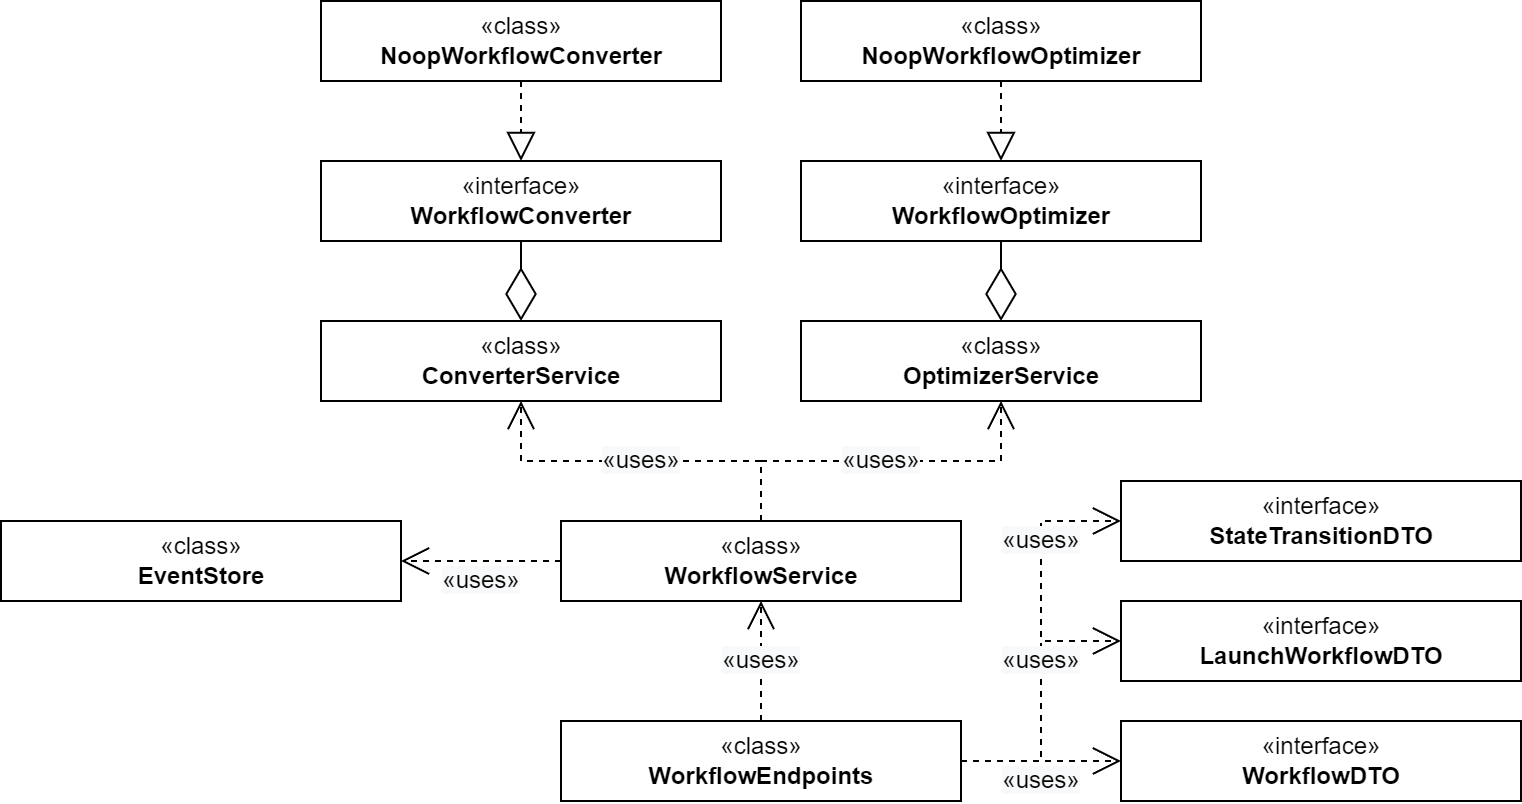
\includegraphics[width=1\textwidth]{proposed-concept/graphics/workflow-module-class-diagram.drawio.png}}
    \caption{UML class diagram of the workflow module of a prototypical \gls{ttsm}.}
    \label{fig:prototype:workflow_module_class_diagram}
\end{figure}

The \textit{WorkflowEndpoints} class also generates a fully fetched OpenAPI definition that is rendered with \textit{Redoc}\footnote{\url{https://github.com/Redocly/redoc} (accessed on 2022-10-29)}, a web-based tool, that creates beautiful single page applications that group and describe exposed endpoints in detail. Generally speaking, the \textit{WorkflowEndpoints} class receives HTTP REST commands with endpoint-specific payloads in the form of \glspl{dto}\footnote{Notice that all \glspl{dto} are marked as interfaces in figure~\ref{fig:prototype:workflow_module_class_diagram}. This is a peculiarity of the chosen programming language, TypeScript. After compiling TypeScript to JavaScript, the interfaces no longer exist because JavaScript is a dynamically typed language, and TypeScript, in contrast, is a statically typed one. Using interfaces instead of classes is, therefore, an optimization that reduces the final application size.}. These \glspl{dto} are then converted and fed forward to the \textit{WorkflowService}. Employing such a conversion allows the definition of multiple, independent endpoint classes, where each endpoint class might satisfy different specifications. This further simplifies the integration of existing solutions since the \textit{WorkflowService} class independently works with entities instead of \glspl{dto}. The endpoints exposed by the \textit{WorkflowEndpoints} class, which allow the definition of new workflows, are listed and briefly described in table~\ref{tab:ttsm:prototype:workflow_definition_endpoints}.

\begin{table}[h]
\centering
\begin{tabular}{|l|l|l|}
    \hline
    \textbf{Method} & \textbf{Path} & \textbf{Description}\\
    \hline
    POST & /workflows & Creates a new workflow and its statecharts.\\
    GET & /workflows & Returns all workflows.\\
    GET & /workflows/\{id\} & Returns the workflow with the given ID.\\
    POST & /workflows/\{id\}/launch & Launches a new instance of a workflow.\\
    \hline
\end{tabular}
\caption{List of workflow definition endpoints}
\label{tab:ttsm:prototype:workflow_definition_endpoints}
\end{table}

Based on the concept of separation between workflow definitions and workflow instantiations in section~\ref{sec:ttsm:proposal:distinction_workflows_instantiations}, workflows must be defined before they can be launched. All \textit{GET} endpoints also allow time travel by supporting an additional query parameter called \textit{until} that must be supplied with an ISO-based timestamp~\cite{iso_timestamps}. With this utility, participants can trace a workflow definition's progress, for example. Similar endpoints are exposed for workflow instantiations listed in table~\ref{tab:ttsm:prototype:workflow_instance_endpoints}.

\begin{table}[h]
\centering
\begin{tabular}{|l|l|l|}
    \hline
    \textbf{Method} & \textbf{Path} & \textbf{Description}\\
    \hline
    GET & /instances & Returns all instances.\\
    GET & /instances/\{id\} & Returns the instance with the given ID.\\
    GET & /instances/\{id\}/payloads & Returns all payloads of a particular instance.\\
    POST & /instances/\{id\}/advance & Performs a state transition.\\
    \hline
\end{tabular}
\caption{List of workflow instance endpoints}
\label{tab:ttsm:prototype:workflow_instance_endpoints}
\end{table}

After a workflow definition is launched, a workflow instantiation is created. This workflow instantiation, and its progress, can also be queried using time travel. To further advance a workflow instantiation (i.e.,\ to perform a state transition), the participant calls the \textit{advance} endpoint on the appropriate instance.

Newly created workflow definitions, instantiations, or state transitions, are then forwarded to the \textit{WorkflowService}. This service contains the actual logic of the workflow module. Since, technically, it should be possible to not only allow statecharts for workflow definitions but also \gls{bpmn} or choreography diagrams, the \textit{WorkflowService} has to choose an applicable converter. Once the workflow definition was forwarded through the \textit{WorkflowService} to the \textit{ConverterService}, the \textit{ConverterService} determines\footnote{By reading a flag that participants have to add to the workflow definition configuration.} in which format the workflow is defined and selects the correct converter strategy. The converter then outputs statecharts, where semantics are the same as the ones previously defined by the participant. Therefore, the prototype internally only ever has to work with statecharts rather than supporting a heterogeneous set of workflow definition languages. Even though it has been proven that transformations from different process definition models to statecharts are possible~\cite{sequence_diagrams_to_statecharts,inter_organizational_bps_managed_by_blockchain}, this prototype only implements the \textit{NoopWorkflowConverter} strategy that inputs statecharts and immediately, without any further transformations, outputs it. This is due to the complexity associated with converter algorithms; however, it shows the feasibility that different strategies could be supported. The algorithm for determining which converter to use is given in algorithm~\ref{alg:ttsm:prototype:choosing_converter_strategy}.

\begin{algorithm}
\caption{Choosing a converter strategy}
\label{alg:ttsm:prototype:choosing_converter_strategy}
\KwIn{A workflow definition configuration $w$, and a list of converters $C$}
\ForAll{$c \in C$}
{
    \If{$w_{type} = c_{type}$}
    {
        \Return{$c(w)$\;}
    }
}
\Return{$null$\;}
\end{algorithm}

In the algorithm implemented, $c_{type}$ represents the supported input type of the converter, and $w_{type}$ is the type specified by the participant for this particular workflow definition. After the conversion is complete, the \textit{WorkflowService} forwards the generated statecharts to the \textit{OptimizerService}. This service then picks the appropriate optimizer strategies, which are also part of the workflow definition configuration. However, compared to the \textit{ConverterService}, the \textit{OptimizerService} might not only perform a single optimization algorithm but multiple in a specified order (total ordering is guaranteed by the proposed \gls{ttsm} concept). The algorithm for this process is defined in the concept in section~\ref{sec:ttsm:proposal:from_workflow_models_to_statecharts} in algorithm~\ref{alg:ttsm:proposal:ordering_optimizers}. An exemplary definition of a simple pedestrian traffic light workflow with appropriate configuration is given in listing~\ref{lst:ttsm:prototype:pedestrian_traffic_light_config}.\\

\begin{lstlisting}[language=json,caption=Exemplary workflow definition of a pedestrian traffic light,captionpos=b,label=lst:ttsm:prototype:pedestrian_traffic_light_config]
{
  "config": {
    "optimizer": ["noop"],
    "type": "STATECHARTS"
  },
  "workflow": {
    "initial": "green",
    "states": {
      "green": { "on": { "TIMER": "red" } },
      "red": { "on": { "TIMER": "green" } }
    }
  }
}
\end{lstlisting}

The prototype only supports the \textit{NoopWorkflowOptimizer}. It immediately returns the input statecharts without modifications to show the feasibility of this multi-optimizer approach. Similar to the converter, optimizers are also rather complex and, therefore, out of scope of this work.

The generated statecharts are then fed into the \textit{XState} library to verify their syntactic and semantic validity. The library is used to depict the current state of a workflow instance and enables ``stateless'' state transitions. In the context of a \gls{ttsm}, this means that the workflow module only has to store the workflow model in the form of statecharts, as generated by the converter and the optimizer, and the current state of the workflow instance. Note that this ``statelessness'' also allows easy reconstruction of previous state machines by time-travelling and extracting the state at another point in time. If a participant wants to perform a state transition, the state machine is reconstructed by the \gls{ttsm} by feeding the workflow model and the current state into \textit{XState}. If the state transition on the reconstructed state machine fails, the workflow module responds with an error.

After conversion, optimization, and validation of workflow definitions, instantiations, and state transitions, the workflow module, and in this case the \textit{WorkflowService} in particular, dispatches a single follow-up event to the persistence module by directly connecting to the event bus of \textit{EventStoreDB}. The list of events is given below:

\begin{itemize}
    \item \textbf{Client.Workflow.Propose}: The participant wants to propose a new workflow definition for the entire network. This event includes the converted and optimized statecharts.
    \item \textbf{Client.Instance.Launch}: The participant wants to launch a new instance of a previously proposed and accepted workflow definition.
    \item \textbf{Client.Instance.Advance}: The participant wants to perform a state transition on a previously launched and accepted workflow instance.
    \item \textbf{Client.Instance.TransitionAccepted}: Some participant wants to perform a state transition, and the state machine has already incorporated it locally.
    \item \textbf{Client.Instance.TransitionFailed}: Some participant wants to perform a state transition, but the local state machine rejects it due to syntactic or semantic errors.
\end{itemize}

The connection to the event bus is also used inside the \textit{WorkflowService} to create projections of the dispatched events. These projections accumulate all events until a certain point in time (thus enabling time travel) and return the state of a particular workflow definition or instantiation.


\subsection{Persistence Module}
\label{sec:ttsm:prototype:persistence_module}
The persistence module, as mentioned afore, is an implicit module that is created by the external \textit{EventStoreDB} system. Modules that need to communicate with the event bus or the event store directly connect using the provided \textit{EventStoreDB Client}\footnote{\url{https://npmjs.com/package/@eventstore/db-client} used in version 3.4.0 (accessed on 2022-11-29)}. The client comes with full TypeScript type support and exposes a list of database command and query functions that are executed using gRPC\footnote{\url{https://grpc.io/} (accessed on 2022-09-06)}, an open source framework for remote procedure calls that is optimized for performance and throughput. To write new events to the event bus, the client provides the \textit{appendToStream} function. This function takes the name of the stream and a JSON-based payload (the event) that should be dispatched. The prototype generates an entirely new stream for each newly defined workflow definition with the name \textit{workflows.\{id\}}, to which associated events are appended. This increases performance because the overall stream size is reduced and makes reading and generating projections easier. The system does not have to filter for events with specific workflow IDs but, instead, can consume the entire stream at once. A similar mechanism has been employed for workflow instantiations. The prototype generates a new stream with the name \textit{instances.\{id\}} for each newly launched workflow instance. The IDs used for workflow definitions and instantiations are generated on the client side using UUIDv4.

Another important concept that the \gls{ttsm}-prototype heavily relies on are projections. To create projections, the \textit{EventStoreDB} client exposes the function \textit{createProjection} that inputs a unique projection name and the projection source code in the form of simplified JavaScript. Projections are typically executed for each new event dispatched to the stream it relies upon. These events are then accumulated\footnote{Imagine an event called \textit{increaseByOne} that is dispatched by some client on an irregular basis. A projection that should count the total amount would then be initialized with value $0$ and adds $1$ to the current value each time this event has been recognized.} over time and stored in a so-called \textit{materialized view}. Figure~\ref{fig:ttsm:prototype:persistence_module_architecture} shows the basic architecture and interaction between an external connector and the \textit{EventStoreDB} itself. The unidirectional arrows denote message flow direction.

\begin{figure}[h]
    \makebox[\textwidth][c]{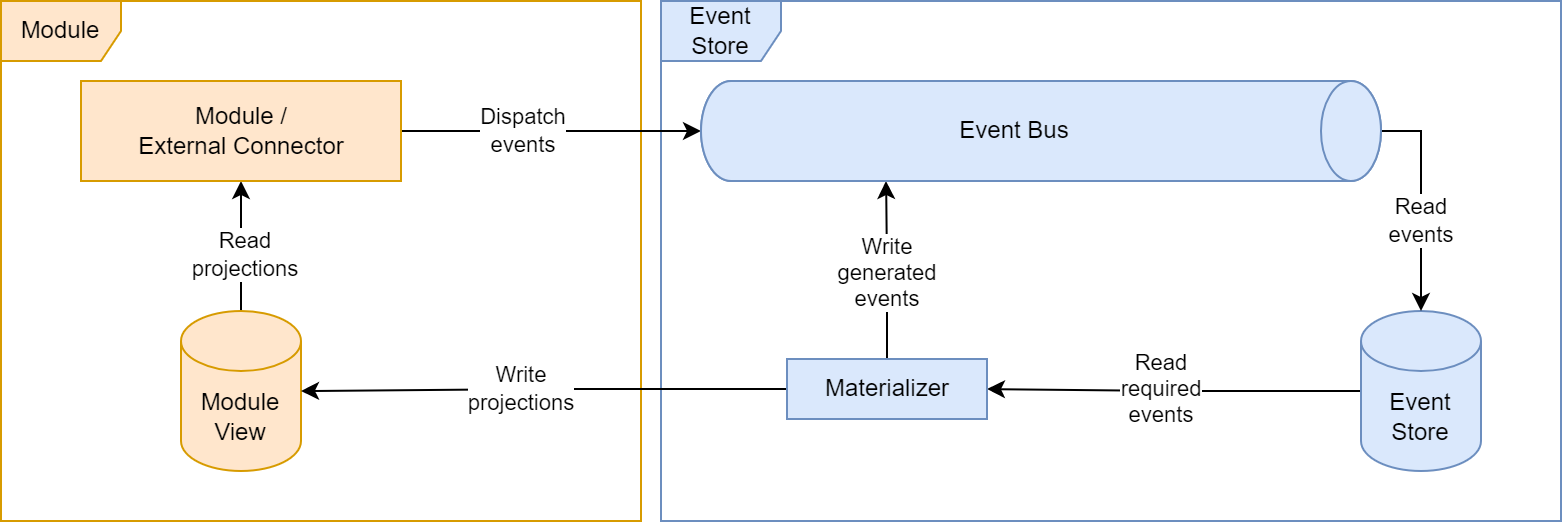
\includegraphics[width=1\textwidth]{proposed-concept/graphics/event-store-architecture.drawio.png}}
    \caption{Persistence module and event store architecture.}
    \label{fig:ttsm:prototype:persistence_module_architecture}
\end{figure}

The event store reads and persists all events dispatched to the event bus and its streams. Since projections are executed on the database side as part of the materializer, events can be directly read from the event store without any network delay involved. Therefore, this prototype could technically be scaled horizontally for large-scale systems by increasing the number of \textit{EventStoreDB} nodes. On the client side, projections generated by the materializer can be queried directly using functions like \textit{getProjectionResult} or subscribed to get notified each time the projection is updated. The second approach is typically the preferred way for event-sourcing systems because projections can be stored directly in appropriate database systems. For example, this might be a relational database system for workflow definitions or an object storage for large data sets like \gls{bim} models. For simplicity reasons, the prototype queries projection results only on demand.

In case a participant, the rules module, or any other potential client needs to verify a previous state, time travel is performed locally in the \gls{ttsm} by accumulating all events from the beginning until a given point in time. This is only possible because the \gls{ttsm} concept guarantees certain properties such as total and causal ordering of events (see section~\ref{sec:ttsm:proposal:capturing_local_progress}), or separation between the persistence of the event history and the current \gls{ttsm}-state~\cite{mistakes_in_event_sourcing}.


\subsection{Rules Module}
\label{sec:ttsm:prototype:rules_module}
This module is similar in structure to the workflow module described in section~\ref{sec:ttsm:prototype:workflow_module}. It uses a three-layer architecture, namely, presentation, application, and data layer. The presentation layer exposes the endpoints used to register external rule validation engines, the application layer performs the asynchronous validation whenever new workflow definitions, workflow instances, or state transitions are received, and the data layer, which persists validation results. These three layers are, once again, loosely coupled by the dependency injection mechanism provided by NestJS\@. Figure~\ref{fig:prototype:rules_module_class_diagram} shows the \gls{uml} class diagram of the rules module.

\begin{figure}[h]
    \makebox[\textwidth][c]{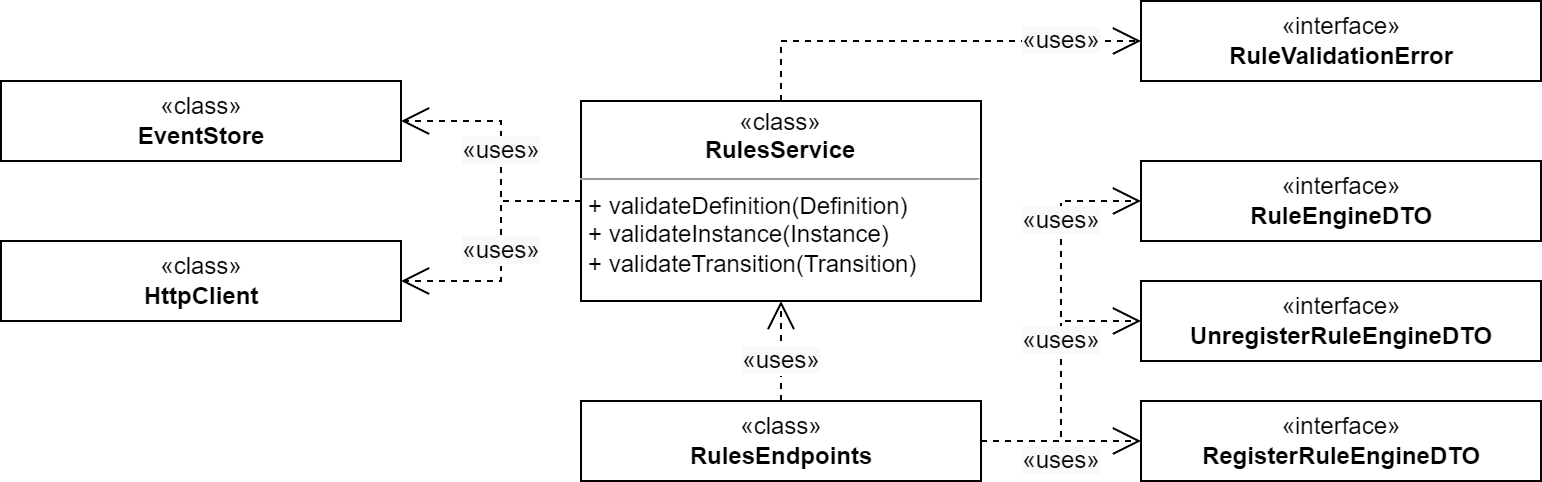
\includegraphics[width=1\textwidth]{proposed-concept/graphics/rules-module-class-diagram.drawio.png}}
    \caption{UML class diagram of the rules module of a prototypical \gls{ttsm}.}
    \label{fig:prototype:rules_module_class_diagram}
\end{figure}

The \textit{RulesEndpoints} class allows a participant that runs a particular instance of the \gls{ttsm} prototype to register rule validation engines that are later on invoked by the \textit{RulesService} if necessary. These engines are used to validate and verify if workflow definitions can be created, workflow instantiations can be launched, and state transitions can be performed under a predefined set of constraints called ``rules''. Furthermore, systems like these are technically able to connect to the persistence module directly and the endpoints exposed by the \textit{EventStoreDB} described in section~\ref{sec:ttsm:prototype:persistence_module}. This enables time-travelling capabilities inside rule validation engines. Thus, state transition and their payloads, for example, can be verified against previous state transitions and payloads\footnote{For example, a facility maintenance contractor has to complete maintenance on an elevator and transmit a document that lists all maintenance steps performed in a predefined structure and order, before the building administrator can perform an inspection. This requires semantic correctness of process execution and the rule validation engines to verify that all required documents are present in the correct form as payloads of previous state transitions.}. The implementation of such rule validation engines and how these kinds of systems let participants define rules are not part of the \gls{ttsm} itself and are out of scope of this work. Therefore, the \gls{ttsm} exposes HTTP REST endpoints that allow the registration of such systems in a loosely coupled fashion. The endpoints supported by this prototype are listed in table~\ref{tab:ttsm:prototype:rules_endpoints}.

\begin{table}[h]
\centering
\begin{tabular}{|l|l|l|}
    \hline
    \textbf{Method} & \textbf{Path} & \textbf{Description}\\
    \hline
    POST & /rules & Registers a new rule service with a callback URL.\\
    GET & /rules & Returns all registered rule services.\\
    GET & /rules/\{id\} & Returns the rule service with the given ID.\\
    PUT & /rules/\{id\} & Updates and changes details of a particular rule service.\\
    DELETE & /rules/\{id\} & Removes a particular rule service.\\
    \hline
\end{tabular}
\caption{List of rules endpoints}
\label{tab:ttsm:prototype:rules_endpoints}
\end{table}

Rule validation engines register themselves at the \gls{ttsm} with a callback URL invoked later on by the \textit{RulesService} to validate commands. The endpoints that rule validation engines must implement in order to be able to interact with the prototype properly are listed in table~\ref{tab:ttsm:prototype:rule_engine_endpoints}.

\begin{table}[h]
\centering
\begin{tabular}{|l|l|l|}
    \hline
    \textbf{Method} & \textbf{Path} & \textbf{Description}\\
    \hline
    POST & /check-new-workflow & Verifies, if the given workflow can be created.\\
    POST & /check-new-instance & Verifies, if the given instance can be launched.\\
    POST & /check-state-transition & Verifies, if the given state transition is allowed.\\
    \hline
\end{tabular}
\caption{List of required rule validation engine endpoints}
\label{tab:ttsm:prototype:rule_engine_endpoints}
\end{table}

As described in sections~\ref{sec:ttsm:proposal:validating_workflow_rules} and~\ref{sec:ttsm:proposal:receiving_commands}, there are two sources of commands that the \textit{RulesService} listens to and sends to all rule validation engines: (1) local commands, that have not yet been transmitted over the network, and (2) the commands received from other participants. In both cases, the \textit{RulesService} subscribes to the event bus of the persistence module in order to properly validate new workflow definitions, instantiations, and state transitions. The command, regardless of its source, is then sent to all rule validation engines registered. Afterwards, the \textit{RulesService} collects all responses and computes the result of the validation and verification process by algorithm~\ref{alg:ttsm:proposal:rules_checking} from section~\ref{sec:ttsm:proposal:validating_workflow_rules}. If the command has been dispatched locally and the result of the validation process is negative, it never enters the network in the first place to prevent blockchain cluttering and to keep a small footprint (see section~\ref{sec:background:on_vs_off_chain:pattern_small_footprint}). If another participant dispatches a command and the validation process is negative, the rules module creates a rejection event. A list of events that are dispatched depending on the results of the validation process is given below:

\begin{itemize}
    \item \textbf{Rules.Instance.LocalTransitionAccepted}: A local state transition has been accepted by all rule validation engines.
    \item \textbf{Rules.Instance.LocalTransitionRejected}: At least one rule validation engine has rejected a local state transition.
    \item \textbf{Rules.Instance.ReceivedTransitionAccepted}: All local rule validation engines have accepted a state transition proposed by another participant.
    \item \textbf{Rules.Instance.ReceivedTransitionRejected}: At least one local rule validation engine has rejected a state transition proposed by another participant.
\end{itemize}

Similar events are dispatched for workflow definitions and workflow instantiations. Note that, as described in the concept in section~\ref{sec:ttsm:proposal:receiving_commands}, participants that dispatch a command (like a state transition, for example) do have to validate it twice, once as a local command and the second time after receiving it through the network. This is because all commands are dispatched to all involved participants. This includes the sender of the command as well. Figure~\ref{fig:prototype:rules_module_flowchart} illustrates the decision-making process of the rules module on which event has to be dispatched as a response.

\begin{figure}[h]
    \makebox[\textwidth][c]{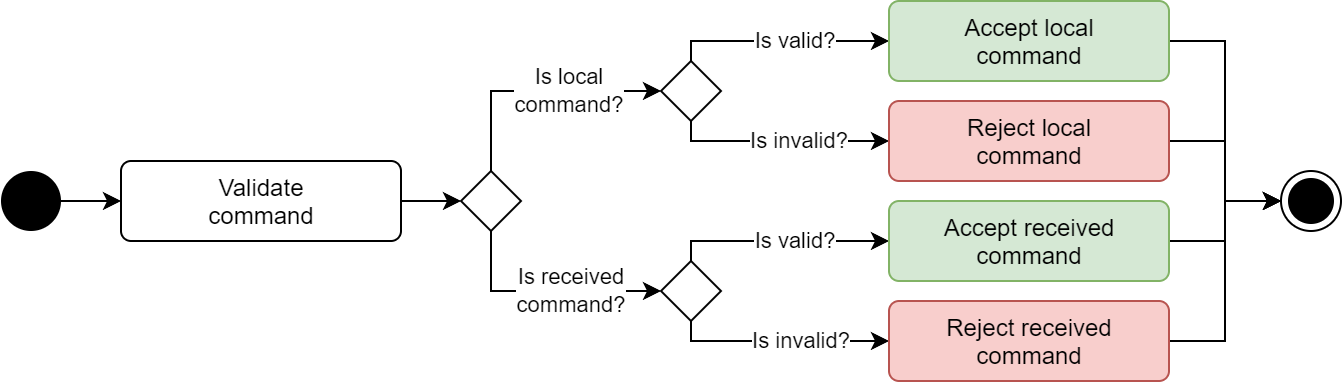
\includegraphics[width=1\textwidth]{proposed-concept/graphics/rules-module-flowchart.drawio.png}}
    \caption{UML flowchart diagram of the rules modules decision-making process.}
    \label{fig:prototype:rules_module_flowchart}
\end{figure}

Since the prototype implements the communication with rule validation engines using HTTP, unexpected network timeouts might occur. In this case, the prototype immediately rejects the command, regardless of the response of other rule validation engines, to prevent the command from being accepted that would otherwise have been rejected. This is a design decision made in the prototype since the \gls{ttsm} concept explicitly delegates the handling of network errors to the implementation (see section~\ref{sec:ttsm:proposal:reaching_consensus}). The dispatched events are then further processed by the consistency module.


\subsection{Consistency Module}
\label{sec:ttsm:prototype:consistency_module}
The consistency module, responsible for exchanging messages between participants, is implemented in this prototype using two layers: (1) the application layer being responsible for determining if a message has to be exchanged, and if so, which consistency strategy to use, and (2) the data layer that directly connects to the \textit{EventStoreDB} to listen for events triggering message exchanges. Figure~\ref{fig:ttsm:prototype:consistency_module_class_diagram} depicts the architecture of the consistency module.

\begin{figure}[h]
    \makebox[\textwidth][c]{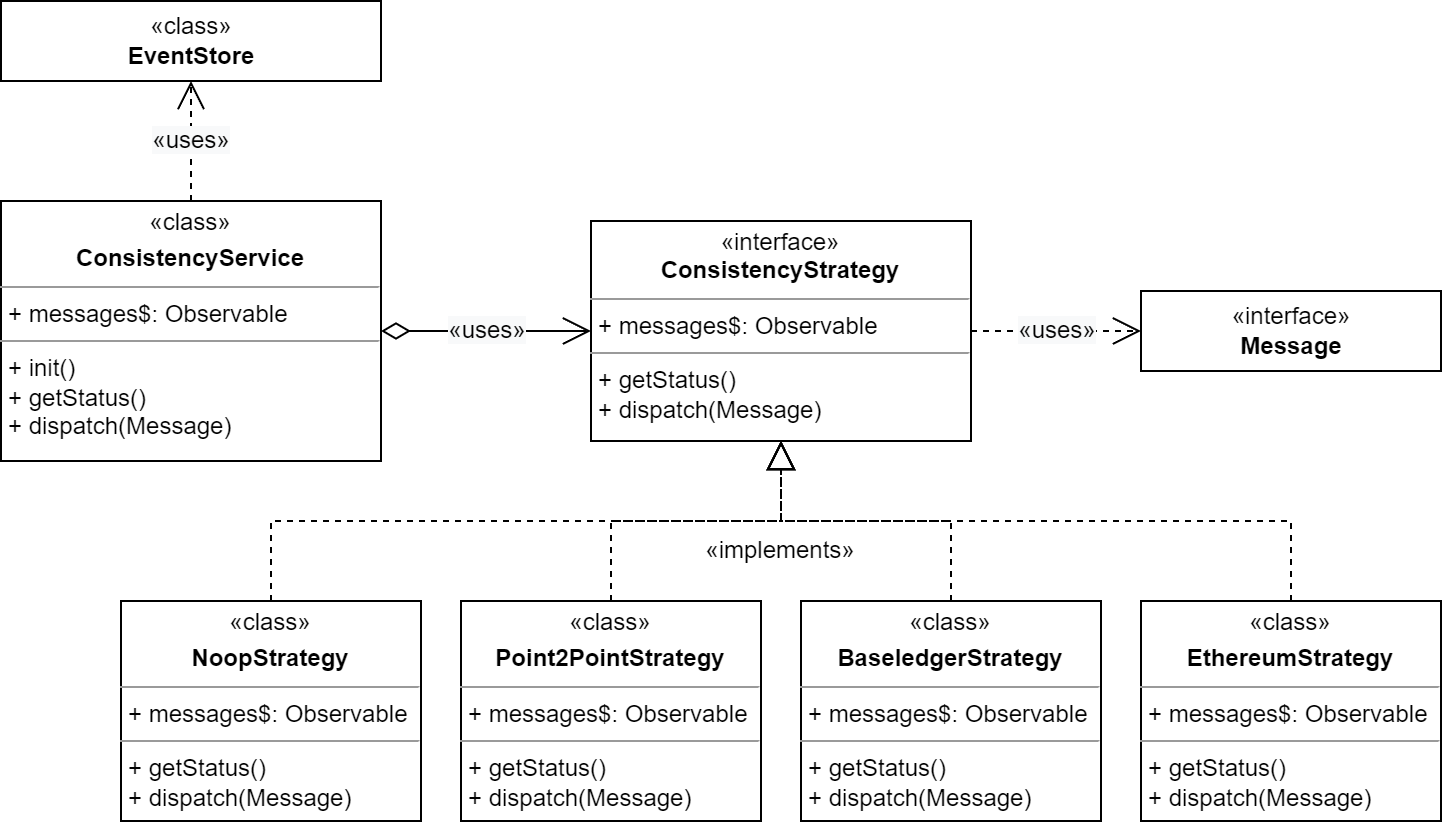
\includegraphics[width=1\textwidth]{proposed-concept/graphics/consistency-module-class-diagram.drawio.png}}
    \caption{Consistency module architecture that enables multi-chain support.}
    \label{fig:ttsm:prototype:consistency_module_class_diagram}
\end{figure}

As described in the proposed concept in section~\ref{sec:ttsm:proposal:entering_blockchain_and_distributing_commands}, the consistency module receives approval events from the rules module through the persistence module. Depending on the persistence event received, an applicable consistency message is generated. In this prototypical implementation, this is accomplished by the \textit{ConsistencyService}, which subscribes to the event bus. In a fully-fledged \gls{ttsm} implementation, the \textit{ConsistencySerivce} would now pick an appropriate \textit{ConsistencyStrategy} depending on implementation-specific metrics such as payload structure or consistency message type. However, to keep the complexity of this prototype design at a reasonable scale, the \textit{ConsistencyStrategy} that is being used is predefined on start-up by the developer. This approach might even be sufficient for most \gls{ttsm} implementations.

Consistency strategies require at least two functions and one field to be implemented. Each consistency strategy implementation has to provide the \textit{messages\$} field that implements the observer pattern and emits a new message for each message sent to other participants. It, therefore, represents a constant and congruent stream in each participant's \gls{ttsm}. The \textit{getStatus} function that returns the status of all required external services (in the case of Ethereum, for example, the status of the node used to write to the blockchain), and the \textit{dispatch(Message)} function that distributes the given message to all participants involved. Some strategies are rather specific, like the \textit{NoopStrategy}, which immediately feeds back the message to the sender (i.e.,\ it can only be used for consistency messages that involve exactly one participant), or the \textit{Point2PointStrategy} that uses HTTP to exchange messages with other participants. A potential use case for the latter one might be the distribution of messages between participants that are not in a conflict of interest, for example. However, most of the communication relies on \gls{bct}-based strategies. How these strategies are implemented and what properties these have to fulfill is out of scope of this work. Nonetheless, they are obligated by the \gls{ttsm} to exchange dispatched messages with other workflow participants reliably and to provide a consistent view of workflows throughout all participants. In this prototypical implementation, \gls{bct}-based strategies are primarily implemented in a rather simplistic way. % chktex 36

\begin{itemize}
    \item The \textbf{\textit{EvmStrategy}} generates a smart contract that only stores hashes of the exchanged messages and returns the transaction address as commitment reference. The messages themselves are exchanged using an HTTP-based REST API\@. It is forwarded to other participants only if the hash was written successfully to the smart contract and, depending on the execution mode, if the commitment reference was attached.
    \item The \textbf{\textit{BaseledgerStrategy}} works in a pretty similar fashion; however, most of the implementation of this strategy is part of the external \textit{baseledger proxy}\footnote{\url{https://github.com/Baseledger/baseledger-proxy} (accessed on 2022-09-07)}. Baseledger implements the Baseline Protocol. As described in section~\ref{sec:background:baseline_protocol}, baseledger uses an internal message bus (in this case NATS\footnote{\url{https://nats.io/} (accessed on 2022-09-07)}, a message bus for the edge) to exchange messages between participants. A \gls{zkp} is generated as a commitment reference and written to the blockchain, proving that the message was dispatched and distributed correctly.
\end{itemize}

Once the command that was converted to a consistency message has been distributed to all involved participants using the chosen consistency strategy, the \textit{ConsistencyService} receives the dispatched message (this includes the \textit{ConsistencyService} of the sender as well - no distinction between sender and receiver has to be made from here on out). The message is then converted from a consistency message transmitted over the network and exchanged between participants to an internal persistence event. Afterwards, the persistence event (and the associated command) is evaluated and validated by the rules and the workflow module for syntactic, semantic, and workflow-specific pragmatic correctness as mentioned in the proposed concept in section~\ref{sec:ttsm:proposal:receiving_commands}. As soon as all involved modules have given their feedback, the \textit{ConsistencyService} dispatches another event into the network that indicates that this \gls{ttsm} either accepts or rejects the command. All participants must wait until $N$ responses were dispatched into the network from $N$ involved participants. If one of these $N$ participants rejects the command, it is immediately rolled back. Figure~\ref{fig:ttsm:prototype:consistency_module_sequence_diagram} shows the simplified network communication between two participants exchanging messages using the \gls{ttsm} prototype.

\begin{figure}[h]
    \makebox[\textwidth][c]{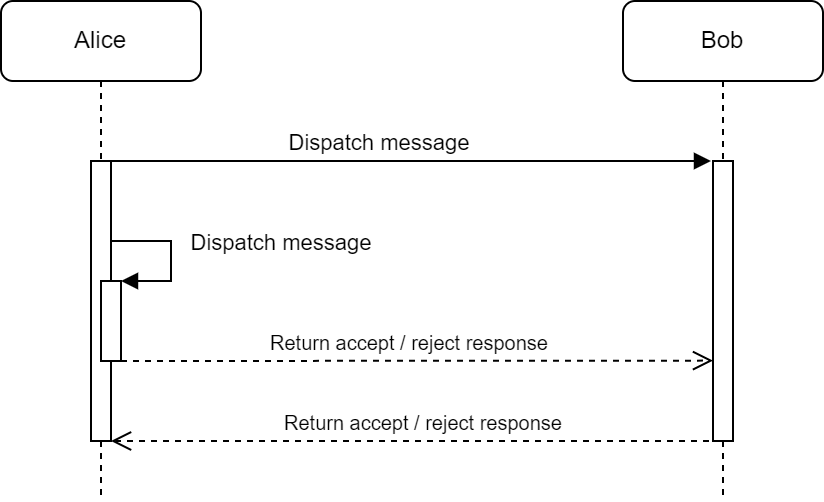
\includegraphics[width=0.8\textwidth]{proposed-concept/graphics/consistency-module-message-exchange.drawio.png}}
    \caption{Sequence diagram of two participants exchanging messages using the consistency module.}
    \label{fig:ttsm:prototype:consistency_module_sequence_diagram}
\end{figure}

The consistency messages required to perform state transitions are listed below\footnote{Similar messages are exchanged for new workflow definitions or instantiations.}. Each message, as shown in figure~\ref{fig:ttsm:proposal:consistency_message_format} in section~\ref{sec:ttsm:proposal:entering_blockchain_and_distributing_commands} consists of a message header and an arbitrary payload that is extended by message and command specific metadata.

\begin{itemize}
    \item \textbf{Perform Transition}: Some participant wants to perform a state transition on a given workflow instance. The metadata consists of the name of the state transition (unique identifier), the starting state, and the resulting state.
    \item \textbf{Accept Transition}: Response message of participants if they accept the state transition. Contains the same metadata as the \textit{perform transition} message.
    \item \textbf{Reject Transition}: Response message of participants if their workflow or rules module produced an error while evaluating the state transition. Contains the same metadata as the \textit{perform transition} message.
\end{itemize}

If an accept or reject message is received, a follow-up persistence event is dispatched by the \textit{ConsistencyService} to allow an examination of participants who rejected and accepted the command. After all responses have been collected, a completion persistence event is emitted as described in algorithm~\ref{alg:ttsm:proposal:consensus} in section~\ref{sec:ttsm:proposal:reaching_consensus}. It is used to allow the consistency module to itself determine when consensus between participants is reached. The persistence events dispatched by the \textit{ConsistencyService} are given below\footnote{Similar persistence events are dispatched for new workflow definitions or instantiations proposed by other participants.}:

\begin{itemize}
    \item \textbf{Consistency.Instance.TransitionReceived}: Created from \textit{perform transition} consistency messages and only dispatched if the workflow instance on which the transition should be performed upon and its workflow definition exist locally.
    \item \textbf{Consistency.Instance.TransitionAcceptedByParticipant}: Created from \textit{accept transition} consistency messages if any of the involved participants approve the state transition.
    \item \textbf{Consistency.Instance.TransitionRejectedByParticipant}: Created from \textit{Reject Transition} consistency messages if any of the involved participants could not perform the state transition due to some issues.
    \item \textbf{Consistency.Instance.TransitionAccepted}: Dispatched by the \textit{ConsistencyService}, if for all $N$ participants involved in the state transition, a \textit{Consistency.Instance.TransitionAcceptedByParticipant} persistence event has been dispatched.
    \item \textbf{Consistency.Instance.TransitionRejected}: Dispatched by the \textit{ConsistencyService}, if for any of the $N$ participants involved in the state transition, a \textit{Consistency.Instance.TransitionRejectedByParticipant} persistence event has been dispatched.
\end{itemize}

To dispatch persistence events, the \textit{ConsistencyService} connects to \textit{EventStoreDB} in the same fashion as the workflow and rules modules do. This includes creating projections (if necessary) and writing workflow definition events to the \textit{workflows.\{id\}} stream and workflow instance events, like state transitions, to the \textit{instances.\{id\}} stream.



\section{Intrinsic Properties}
\label{sec:ttsm:properties}
The knowledge accumulated in the background section~\ref{sec:background}, together with the research conducted to extract related work in section~\ref{sec:related-work}, led to a new concept for workflow execution that leverages on \glspl{bct} for verifiability and traceability. This concept, as described in detail in section~\ref{sec:ttsm:proposal}, and its prototypical implementation described in section~\ref{sec:ttsm:prototype} gave a sophisticated overview of properties that \glspl{ttsm} that allow time-travel verification of executed workflows need to fulfill to be viable. The following lists five distinct properties derived from the concept and the implemented prototype and describes them in more detail.

\subsubsection{Consistent}
\label{sec:ttsm:properties:consistent}
The \textit{consistency property} guarantees that all participants \textit{eventually} reach consensus and work with the exact same state for all workflows being defined or executed. As described at the beginning of section~\ref{sec:ttsm:proposal}, this property is partially enabled by the involved \glspl{bct} because their consensus protocols must guarantee at least agreement, integrity, and termination when exchanging messages and advancing the state of a blockchain (see section~\ref{sec:background:blockchain:consensus-protocols}). The \gls{ttsm}-consensus algorithm described in section~\ref{sec:ttsm:proposal:reaching_consensus} shows that the \gls{ttsm} itself can also reach consensus between all involved participants, leveraging on the aforementioned properties that \glspl{bct} and their consensus protocols bring to the table. However, due to the increased block time of certain blockchains, consistency can only be archived in the form of \textit{eventual consistency}. Nonetheless, \glspl{ttsm} that have reached finality can never be inconsistent. If participants, for example, request invalid state transitions, they are rejected immediately, which forces everyone involved to roll back. A similar scenario occurs if two or more participants aim to perform the same state transition simultaneously. Because these participants already locally advanced their state, the same transition cannot be performed twice. Even though the state transition is technically idempotent, the \gls{ttsm} still rolls back due to potentially diverging payloads. This is ensured by the workflow logic, the persistence module, and the \gls{bct} itself.

\subsubsection{Persistent}
\label{sec:ttsm:properties:persistent}
All changes performed within a \gls{ttsm} and messages exchanged between participants must be available in the form of an event history. This is referred to as the \textit{persistency property}. Persistence in the context of a \gls{ttsm} is two-fold: (1) the event bus and the event store of each participant are responsible for persisting all exchanged messages and internal \gls{ttsm} events. Since hostile participants could technically modify this data in their favor, (2) the \glspl{bct} also store certain proofs of messages that have been exchanged. Even if a hostile participant tampers their data, the other participants still have undeniable proof that specific actions have been performed. This splits persistence into two distinct areas of concern:

\begin{itemize}
    \item \textbf{Tamper-proofness}: Hinders hostile participants to change workflow execution in their favor in hindsight and generates undeniable proof (see section~\ref{sec:ttsm:proposal:entering_blockchain_and_distributing_commands}).
    \item \textbf{Storage}: Enables participants to execute large workflows with varying payloads on public blockchains without exposing privacy critical information (see section~\ref{sec:ttsm:proposal:capturing_local_progress}) and reducing the footprint on the blockchain, which reduces overall cost (see section~\ref{sec:background:on_vs_off_chain:pattern_small_footprint}).
\end{itemize}

Both properties are tightly coupled in a \gls{ttsm} to give participants access to persistence proofs on the blockchain. Due to the employed design principles of the persistence and consistency modules (such as \gls{cqrs}, event sourcing, or causal ordering), invalid commands can never become a part of the eventually consistent state of a workflow or even the entire system. Such commands are stored in the event history for traceability reasons, but are never incorporated into the state.

\subsubsection{Verifiable}
\label{sec:ttsm:properties:verifiable}
Whenever multiple participants in a conflict of interest are involved in the execution of a workflow, the \textit{verifiability property} is of utmost importance because it gives proof that certain events have happened in a particular order at a certain point in time. This property is tightly coupled with the aforementioned \textit{consistency property}~\ref{sec:ttsm:properties:consistent} and the \textit{persistency property}~\ref{sec:ttsm:properties:persistent}. Even though hostile participants might modify their local state, the global state, which is stored to some extent on the blockchain, cannot be tampered with\footnote{Given, that the underlying \gls{bct} has enough participants and implements a proper consensus protocol~\cite{public_chains_make_private_chains_obsolete}.}. If participants want to prove that some action happened in the past, they can go back in time using the time-travelling capabilities of the \gls{ttsm} and access the proof on the blockchain associated with the events. Even though not all events might be incorporated into the current system state, they are still part of the event history and hence something participants can verify. Therefore, verifiability is once again a property backed by the underlying \gls{bct} and leveraged upon in the proposed concept of a \gls{ttsm}. The consistency property ensures that the state is consistent in the first place, which guarantees that verification produces the same results for all participants, while the persistency property enables time travel which allows the verification of past states.

\subsubsection{Declarative}
\label{sec:ttsm:properties:declarative}
In order to keep development cost in case of changing requirements at a minimum, and to allow management-oriented users to define new workflows, a \gls{ttsm} has to fulfill the \textit{declarative property}. Being declarative means that users of a \gls{ttsm} can entirely configure the execution of workflows without the need for additional software development effort\footnote{An example of such a configuration is given in listing~\ref{lst:ttsm:prototype:pedestrian_traffic_light_config} in the prototype design section~\ref{sec:ttsm:prototype}.}. Being configurable and purely declarative not only enables software architects to use \glspl{ttsm} as underlying sources of truth for workflow execution, but it also simplifies the integration into existing systems. As described in sections~\ref{sec:ttsm:proposal:from_workflow_models_to_statecharts} and~\ref{sec:ttsm:prototype:workflow_module}, fully-fledged \glspl{ttsm} might not only support statecharts as the language of workflow modeling but also \gls{bpmn}, choreography or even process diagrams. Supporting well-established modeling languages further improves the practical value of such a system.

\subsubsection{Optimized}
\label{sec:ttsm:properties:optimized}
Due to highly fluctuating transaction fees of blockchains, the \gls{ttsm} should reduce the number of messages exchanged to also reduce overall cost~\cite{predicting_cryptocurrency_price_bubbles}. This is referred to as the \textit{optimization property} and is enabled by the optimizer described in section~\ref{sec:ttsm:proposal:from_workflow_models_to_statecharts} of the proposed concept. Optimizing workflow statecharts can change the syntactic meaning of workflows; however, they must preserve semantics.


\subsection{Research Question 2}
\label{sec:ttsm:properties:rq2}
To answer the second research question:

\begin{quote}
    \emph{Which properties do \gls{bct}-based state machines require to allow time-travel verification of business processes?}
\end{quote}

As mentioned above, blockchains already support a vast majority of properties required in \gls{bct}-based state machines that allow time-travel verification. However, most related work (as described in section~\ref{sec:related-work:comparison}) leverages on these properties by directly executing workflows on the blockchain. Even though tamper-proofness and consistency are assured, these approaches suffer from a lack of privacy-preserving mechanisms, longer transaction times, a lack of blockchain-acquainted developers, or restrictions to the payload size\footnote{Primarily due to native block size limits.}. Therefore, the set of properties defined for the concept proposed in this work tries to leverage on characteristics of \glspl{bct} without creating tight coupling between the blockchain and the workflow execution engine. Properties that \glspl{ttsm} \textbf{must} fulfill in order to be fully functional and to allow time-travel verification of business processes are: (1) the \textit{consistency property}, that ensures that eventually, all participants read the same state of a workflow execution, (2) the \textit{persistency property}, that stores the state in an undeniable and tamper-proof fashion without exposing privacy critical information to uninvolved participants and (3) the \textit{verifiability property}, that enables traceability through time-travel. Properties that \textbf{should} be fulfilled in order to make the concept suitable for real-world scenarios are the (1) \textit{optimization property} and (2) the \textit{declarative property}.

Nonetheless, the question remains on how the state of the art must be adapted to fulfill these properties and if integrating a \gls{ttsm} in existing systems is viable. Therefore, the upcoming sections evaluate the concept by using analytical and architectural analysis and by investigating its utility in simplified real-world scenarios.



% \subsection{Outline of the time-travelling state machine proposal}
% \begin{itemize}
    % \item Business Process / Choreography only configured via JSON or YAML (can be extended arbitrarily) to be more agnostic and keep sub-systems loosely coupled~\cite{interpreted_bp_on_blockchain_loukil}
    % \item Do not include translators because it adds complexity, gives opportunity for another master thesis and allows loose coupling
    % \item Could use state and state transition optimization as proposed by Nakamura et al. using state charts~\cite{inter_organizational_bps_managed_by_blockchain} (out of scope)
    % \item State Machine only communicates and transmits state transitions with payloads (might cause trouble with payload size in some occasions)
    % \item State Machine only writes to the blockchain, that all (relevant) parties have seen (and confirmed) the transmitted payload (2/3 of relevant participants might even be sufficient due to Byzantine fault tolerance)
    % \item State Machine internally uses \textit{Event Sourcing} to keep track of the history of state transitions but does NOT care about data transmitted
    % \item Rule Engine listens to the emitted \textit{Events} and can time-travel
    % \item All (relevant) participants must confirm that they received the business process and that they agree with the proposed state transitions (can be assumed, maybe with configuration hash, but is mostly out of scope)
    % \item Idea for Task and Business Process Design in \cite{lean_architecture_for_blockchain_based_process_execution}
    % \item Consider multi-chain support where each participant might use her own blockchain as proposed in \cite{architecture_for_multi_chain_bp_ladleif} (could be added, but out of scope)
% \end{itemize}

% \subsection{Components of a time-travelling state machine}
% \begin{itemize}
    % \item[\textbf{Consistency-Module}] Handles the communication between participants and is the only module that directly talks to the blockchain. Uses the strategy design pattern\footnote{\url{https://en.wikipedia.org/wiki/Strategy_pattern}} to integrate other forms of communication (e.g. signature-based, NOOP-strategies, smart contract strategies, etc.).
    % \item[\textbf{Persistence-Module}] Persists all events that ever occurred and exposes state for any point in time (e.g. integration of Kafka, RabbitMQ, EventSourceDB, etc.)
    % \item[\textbf{Optimizer-Module}] Optimizes communication using reduction algorithms for the configuration as mentioned here \cite{inter_organizational_bps_managed_by_blockchain}.
    % \item[\textbf{Workflow-Module}] Handles the advancement of the business process and ensures that state transitions comply with defined ``rules''. External services or sub-components could be used that make use of the time-travelling aspect of the persistence module to check if state transitions are allowed (e.g. integration of an external rule engine).
% \end{itemize}

% \subsection{Ideas during implementation}
% \begin{itemize}
    % \item All events must be idempotent because the sender will also receive all her own events (and they are now ;-)
    % \item Consistency module only depends on the persistence module and workflow module only writes into persistence module
    % \item Commitment reference is stored with every consistency event transmitted over the blockchain and is attached to events in the persistence module
    % \item Events in the persistence module are \textbf{NOT} the same as the events in the consistency module. This is due to the fact, that more complex business processes might not want to write every single process step to the blockchain because they are internal only. This surely is a design decision. Because this means, that there can only be at most as many consistency events as there are persistence events. Everything else must be dropped.
    % \item The TTSM implements the CQRS-pattern. This really helps with scalability and improves reads. Improving reads is a wanted attribute because the payload data that is transferred between states can have an arbitrary data structure depending on the use case. Allowing different database technologies for reads can improve performance dramatically (look into pros and cons of CQRS: \url{https://redhat.com/architect/pros-and-cons-cqrs}, \url{https://betterprogramming.pub/cqrs-software-architecture-pattern-the-good-the-bad-and-the-ugly-e9d6e7a34daf})
    % \item Event sourcing and CQRS allows completely asynchronous communication with external services. This means, that the client can advance the state independently from the block transaction time of the blockchain or the response of the rule engine, but has to expect rollbacks.
    % \item Depending on the proposed workflow instance, the consistency module can decide by itself which messages are being exchanged via blockchain and which blockchain strategy to use.
% \end{itemize}

% Jan Ladleif has some interesting NodeJS repositories for BPMN on his GitHub profile \url{https://github.com/jan-ladleif?tab=repositories}.



% \section{Privacy on the Blockchain}
% A lot of cool literature about zero-knowledge proofs, homomorphic encryption and TEE in \cite{blockchain_for_secure_io_bp}
